\documentclass[twoside]{book}

% Packages required by doxygen
\usepackage{fixltx2e}
\usepackage{calc}
\usepackage{doxygen}
\usepackage[export]{adjustbox} % also loads graphicx
\usepackage{graphicx}
\usepackage[utf8]{inputenc}
\usepackage{makeidx}
\usepackage{multicol}
\usepackage{multirow}
\PassOptionsToPackage{warn}{textcomp}
\usepackage{textcomp}
\usepackage[nointegrals]{wasysym}
\usepackage[table]{xcolor}

% Font selection
\usepackage[T1]{fontenc}
\usepackage[scaled=.90]{helvet}
\usepackage{courier}
\usepackage{amssymb}
\usepackage{sectsty}
\renewcommand{\familydefault}{\sfdefault}
\allsectionsfont{%
  \fontseries{bc}\selectfont%
  \color{darkgray}%
}
\renewcommand{\DoxyLabelFont}{%
  \fontseries{bc}\selectfont%
  \color{darkgray}%
}
\newcommand{\+}{\discretionary{\mbox{\scriptsize$\hookleftarrow$}}{}{}}

% Page & text layout
\usepackage{geometry}
\geometry{%
  a4paper,%
  top=2.5cm,%
  bottom=2.5cm,%
  left=2.5cm,%
  right=2.5cm%
}
\tolerance=750
\hfuzz=15pt
\hbadness=750
\setlength{\emergencystretch}{15pt}
\setlength{\parindent}{0cm}
\setlength{\parskip}{3ex plus 2ex minus 2ex}
\makeatletter
\renewcommand{\paragraph}{%
  \@startsection{paragraph}{4}{0ex}{-1.0ex}{1.0ex}{%
    \normalfont\normalsize\bfseries\SS@parafont%
  }%
}
\renewcommand{\subparagraph}{%
  \@startsection{subparagraph}{5}{0ex}{-1.0ex}{1.0ex}{%
    \normalfont\normalsize\bfseries\SS@subparafont%
  }%
}
\makeatother

% Headers & footers
\usepackage{fancyhdr}
\pagestyle{fancyplain}
\fancyhead[LE]{\fancyplain{}{\bfseries\thepage}}
\fancyhead[CE]{\fancyplain{}{}}
\fancyhead[RE]{\fancyplain{}{\bfseries\leftmark}}
\fancyhead[LO]{\fancyplain{}{\bfseries\rightmark}}
\fancyhead[CO]{\fancyplain{}{}}
\fancyhead[RO]{\fancyplain{}{\bfseries\thepage}}
\fancyfoot[LE]{\fancyplain{}{}}
\fancyfoot[CE]{\fancyplain{}{}}
\fancyfoot[RE]{\fancyplain{}{\bfseries\scriptsize Generated by Doxygen }}
\fancyfoot[LO]{\fancyplain{}{\bfseries\scriptsize Generated by Doxygen }}
\fancyfoot[CO]{\fancyplain{}{}}
\fancyfoot[RO]{\fancyplain{}{}}
\renewcommand{\footrulewidth}{0.4pt}
\renewcommand{\chaptermark}[1]{%
  \markboth{#1}{}%
}
\renewcommand{\sectionmark}[1]{%
  \markright{\thesection\ #1}%
}

% Indices & bibliography
\usepackage{natbib}
\usepackage[titles]{tocloft}
\setcounter{tocdepth}{3}
\setcounter{secnumdepth}{5}
\makeindex

% Hyperlinks (required, but should be loaded last)
\usepackage{ifpdf}
\ifpdf
  \usepackage[pdftex,pagebackref=true]{hyperref}
\else
  \usepackage[ps2pdf,pagebackref=true]{hyperref}
\fi
\hypersetup{%
  colorlinks=true,%
  linkcolor=blue,%
  citecolor=blue,%
  unicode%
}

% Custom commands
\newcommand{\clearemptydoublepage}{%
  \newpage{\pagestyle{empty}\cleardoublepage}%
}

\usepackage{caption}
\captionsetup{labelsep=space,justification=centering,font={bf},singlelinecheck=off,skip=4pt,position=top}

%===== C O N T E N T S =====

\begin{document}

% Titlepage & ToC
\hypersetup{pageanchor=false,
             bookmarksnumbered=true,
             pdfencoding=unicode
            }
\pagenumbering{alph}
\begin{titlepage}
\vspace*{7cm}
\begin{center}%
{\Large Grading Assistant }\\
\vspace*{1cm}
{\large Generated by Doxygen 1.8.13}\\
\end{center}
\end{titlepage}
\clearemptydoublepage
\pagenumbering{roman}
\tableofcontents
\clearemptydoublepage
\pagenumbering{arabic}
\hypersetup{pageanchor=true}

%--- Begin generated contents ---
\chapter{Hierarchical Index}
\section{Class Hierarchy}
This inheritance list is sorted roughly, but not completely, alphabetically\+:\begin{DoxyCompactList}
\item \contentsline{section}{Database\+Manager}{\pageref{class_database_manager}}{}
\item \contentsline{section}{Database\+Table}{\pageref{class_database_table}}{}
\item \contentsline{section}{File\+Manager}{\pageref{class_file_manager}}{}
\item \contentsline{section}{G\+A\+Identifiable\+Object}{\pageref{class_g_a_identifiable_object}}{}
\begin{DoxyCompactList}
\item \contentsline{section}{G\+A\+Annotation}{\pageref{class_g_a_annotation}}{}
\item \contentsline{section}{G\+A\+Assignment}{\pageref{class_g_a_assignment}}{}
\item \contentsline{section}{G\+A\+Assignment\+Data}{\pageref{class_g_a_assignment_data}}{}
\item \contentsline{section}{G\+A\+Class}{\pageref{class_g_a_class}}{}
\item \contentsline{section}{G\+A\+Rubric}{\pageref{class_g_a_rubric}}{}
\item \contentsline{section}{G\+A\+Rubric\+Row}{\pageref{class_g_a_rubric_row}}{}
\item \contentsline{section}{G\+A\+Student}{\pageref{class_g_a_student}}{}
\end{DoxyCompactList}
\item \contentsline{section}{Grading\+Assistant}{\pageref{class_grading_assistant}}{}
\item \contentsline{section}{User\+Settings}{\pageref{class_user_settings}}{}
\end{DoxyCompactList}

\chapter{Class Index}
\section{Class List}
Here are the classes, structs, unions and interfaces with brief descriptions\+:\begin{DoxyCompactList}
\item\contentsline{section}{\hyperlink{class_database_manager}{Database\+Manager} }{\pageref{class_database_manager}}{}
\item\contentsline{section}{\hyperlink{class_database_table}{Database\+Table} }{\pageref{class_database_table}}{}
\item\contentsline{section}{\hyperlink{class_file_manager}{File\+Manager} }{\pageref{class_file_manager}}{}
\item\contentsline{section}{\hyperlink{class_g_a_annotation}{G\+A\+Annotation} }{\pageref{class_g_a_annotation}}{}
\item\contentsline{section}{\hyperlink{class_g_a_assignment}{G\+A\+Assignment} }{\pageref{class_g_a_assignment}}{}
\item\contentsline{section}{\hyperlink{class_g_a_assignment_data}{G\+A\+Assignment\+Data} }{\pageref{class_g_a_assignment_data}}{}
\item\contentsline{section}{\hyperlink{class_g_a_class}{G\+A\+Class} }{\pageref{class_g_a_class}}{}
\item\contentsline{section}{\hyperlink{class_g_a_identifiable_object}{G\+A\+Identifiable\+Object} }{\pageref{class_g_a_identifiable_object}}{}
\item\contentsline{section}{\hyperlink{class_g_a_rubric}{G\+A\+Rubric} }{\pageref{class_g_a_rubric}}{}
\item\contentsline{section}{\hyperlink{class_g_a_rubric_row}{G\+A\+Rubric\+Row} }{\pageref{class_g_a_rubric_row}}{}
\item\contentsline{section}{\hyperlink{class_g_a_student}{G\+A\+Student} }{\pageref{class_g_a_student}}{}
\item\contentsline{section}{\hyperlink{class_grading_assistant}{Grading\+Assistant} }{\pageref{class_grading_assistant}}{}
\item\contentsline{section}{\hyperlink{class_user_settings}{User\+Settings} }{\pageref{class_user_settings}}{}
\end{DoxyCompactList}

\chapter{Class Documentation}
\hypertarget{class_database_manager}{}\section{Database\+Manager Class Reference}
\label{class_database_manager}\index{Database\+Manager@{Database\+Manager}}
\subsection*{Public Member Functions}
\begin{DoxyCompactItemize}
\item 
\hyperlink{class_database_manager_afc98bb0ecd0a4acd6094bc2de4a3c0f9}{Database\+Manager} (std\+::string path)
\begin{DoxyCompactList}\small\item\em Create a \hyperlink{class_database_manager}{Database\+Manager}. \end{DoxyCompactList}\item 
\hyperlink{class_database_manager_ae9b3a5da1e04fbb00faf8a034da1d063}{$\sim$\+Database\+Manager} ()
\begin{DoxyCompactList}\small\item\em Deconstruct the \hyperlink{class_database_manager}{Database\+Manager}. \end{DoxyCompactList}\item 
std\+::string \hyperlink{class_database_manager_a623413cf45f53334a7cde7ed030c9620}{get\+\_\+path} ()
\begin{DoxyCompactList}\small\item\em Get the path used to store the database. \end{DoxyCompactList}\item 
void \hyperlink{class_database_manager_aa3d5f606c609705694a7ece8e31cd987}{set\+\_\+path} (std\+::string path)
\begin{DoxyCompactList}\small\item\em Set the path used to store the database. \end{DoxyCompactList}\item 
\mbox{\Hypertarget{class_database_manager_a6c583242d2a2971a285531886d08f377}\label{class_database_manager_a6c583242d2a2971a285531886d08f377}} 
void \hyperlink{class_database_manager_a6c583242d2a2971a285531886d08f377}{open} ()
\begin{DoxyCompactList}\small\item\em Open the database, if it is not already opened. \end{DoxyCompactList}\item 
\mbox{\Hypertarget{class_database_manager_a36c8ab027e11aba2464f384b18e814e5}\label{class_database_manager_a36c8ab027e11aba2464f384b18e814e5}} 
void \hyperlink{class_database_manager_a36c8ab027e11aba2464f384b18e814e5}{close} ()
\begin{DoxyCompactList}\small\item\em Close the database, if it is already opened. \end{DoxyCompactList}\item 
bool \hyperlink{class_database_manager_aa5d35a29bdad47e640622ac6e92efd82}{is\+\_\+open} ()
\begin{DoxyCompactList}\small\item\em Check if the database is open. \end{DoxyCompactList}\item 
sqlite3 $\ast$ \hyperlink{class_database_manager_a596c53099fb11d1cdddcc493c2ccb314}{db} ()
\begin{DoxyCompactList}\small\item\em Get the sqlite3 database reference. \end{DoxyCompactList}\item 
\mbox{\Hypertarget{class_database_manager_a8f991e99913d1fd0f0f4e75fb7261f1d}\label{class_database_manager_a8f991e99913d1fd0f0f4e75fb7261f1d}} 
void \hyperlink{class_database_manager_a8f991e99913d1fd0f0f4e75fb7261f1d}{dberror} ()
\begin{DoxyCompactList}\small\item\em Print the sqlite3 error to cerr. \end{DoxyCompactList}\item 
void \hyperlink{class_database_manager_a6fc3fa295292d8c873abb4a2f4e73e5b}{dberror} (std\+::string message)
\begin{DoxyCompactList}\small\item\em Print a message, and the sqlite3 error to cerr. \end{DoxyCompactList}\end{DoxyCompactItemize}


\subsection{Constructor \& Destructor Documentation}
\mbox{\Hypertarget{class_database_manager_afc98bb0ecd0a4acd6094bc2de4a3c0f9}\label{class_database_manager_afc98bb0ecd0a4acd6094bc2de4a3c0f9}} 
\index{Database\+Manager@{Database\+Manager}!Database\+Manager@{Database\+Manager}}
\index{Database\+Manager@{Database\+Manager}!Database\+Manager@{Database\+Manager}}
\subsubsection{\texorpdfstring{Database\+Manager()}{DatabaseManager()}}
{\footnotesize\ttfamily Database\+Manager\+::\+Database\+Manager (\begin{DoxyParamCaption}\item[{std\+::string}]{path }\end{DoxyParamCaption})}



Create a \hyperlink{class_database_manager}{Database\+Manager}. 

The Database will be opened automatically. Re-\/calling \hyperlink{class_database_manager_a6c583242d2a2971a285531886d08f377}{open()} is ok.


\begin{DoxyParams}{Parameters}
{\em path} & The path used to store the database \\
\hline
\end{DoxyParams}
\mbox{\Hypertarget{class_database_manager_ae9b3a5da1e04fbb00faf8a034da1d063}\label{class_database_manager_ae9b3a5da1e04fbb00faf8a034da1d063}} 
\index{Database\+Manager@{Database\+Manager}!````~Database\+Manager@{$\sim$\+Database\+Manager}}
\index{````~Database\+Manager@{$\sim$\+Database\+Manager}!Database\+Manager@{Database\+Manager}}
\subsubsection{\texorpdfstring{$\sim$\+Database\+Manager()}{~DatabaseManager()}}
{\footnotesize\ttfamily Database\+Manager\+::$\sim$\+Database\+Manager (\begin{DoxyParamCaption}{ }\end{DoxyParamCaption})}



Deconstruct the \hyperlink{class_database_manager}{Database\+Manager}. 

This will close the database. It is ok to \hyperlink{class_database_manager_a36c8ab027e11aba2464f384b18e814e5}{close()} it before deconstruction. 

\subsection{Member Function Documentation}
\mbox{\Hypertarget{class_database_manager_a596c53099fb11d1cdddcc493c2ccb314}\label{class_database_manager_a596c53099fb11d1cdddcc493c2ccb314}} 
\index{Database\+Manager@{Database\+Manager}!db@{db}}
\index{db@{db}!Database\+Manager@{Database\+Manager}}
\subsubsection{\texorpdfstring{db()}{db()}}
{\footnotesize\ttfamily sqlite3 $\ast$ Database\+Manager\+::db (\begin{DoxyParamCaption}{ }\end{DoxyParamCaption})}



Get the sqlite3 database reference. 

\begin{DoxyReturn}{Returns}
The sqlite3 database reference 
\end{DoxyReturn}
\mbox{\Hypertarget{class_database_manager_a6fc3fa295292d8c873abb4a2f4e73e5b}\label{class_database_manager_a6fc3fa295292d8c873abb4a2f4e73e5b}} 
\index{Database\+Manager@{Database\+Manager}!dberror@{dberror}}
\index{dberror@{dberror}!Database\+Manager@{Database\+Manager}}
\subsubsection{\texorpdfstring{dberror()}{dberror()}}
{\footnotesize\ttfamily void Database\+Manager\+::dberror (\begin{DoxyParamCaption}\item[{std\+::string}]{message }\end{DoxyParamCaption})}



Print a message, and the sqlite3 error to cerr. 


\begin{DoxyParams}{Parameters}
{\em message} & The message to print in addition to the sqlite3 error \\
\hline
\end{DoxyParams}
\mbox{\Hypertarget{class_database_manager_a623413cf45f53334a7cde7ed030c9620}\label{class_database_manager_a623413cf45f53334a7cde7ed030c9620}} 
\index{Database\+Manager@{Database\+Manager}!get\+\_\+path@{get\+\_\+path}}
\index{get\+\_\+path@{get\+\_\+path}!Database\+Manager@{Database\+Manager}}
\subsubsection{\texorpdfstring{get\+\_\+path()}{get\_path()}}
{\footnotesize\ttfamily std\+::string Database\+Manager\+::get\+\_\+path (\begin{DoxyParamCaption}{ }\end{DoxyParamCaption})}



Get the path used to store the database. 

\begin{DoxyReturn}{Returns}
The path 
\end{DoxyReturn}
\mbox{\Hypertarget{class_database_manager_aa5d35a29bdad47e640622ac6e92efd82}\label{class_database_manager_aa5d35a29bdad47e640622ac6e92efd82}} 
\index{Database\+Manager@{Database\+Manager}!is\+\_\+open@{is\+\_\+open}}
\index{is\+\_\+open@{is\+\_\+open}!Database\+Manager@{Database\+Manager}}
\subsubsection{\texorpdfstring{is\+\_\+open()}{is\_open()}}
{\footnotesize\ttfamily bool Database\+Manager\+::is\+\_\+open (\begin{DoxyParamCaption}{ }\end{DoxyParamCaption})}



Check if the database is open. 

\begin{DoxyReturn}{Returns}
Whether the database is open or closed 
\end{DoxyReturn}
\mbox{\Hypertarget{class_database_manager_aa3d5f606c609705694a7ece8e31cd987}\label{class_database_manager_aa3d5f606c609705694a7ece8e31cd987}} 
\index{Database\+Manager@{Database\+Manager}!set\+\_\+path@{set\+\_\+path}}
\index{set\+\_\+path@{set\+\_\+path}!Database\+Manager@{Database\+Manager}}
\subsubsection{\texorpdfstring{set\+\_\+path()}{set\_path()}}
{\footnotesize\ttfamily void Database\+Manager\+::set\+\_\+path (\begin{DoxyParamCaption}\item[{std\+::string}]{path }\end{DoxyParamCaption})}



Set the path used to store the database. 

This method will automatically \hyperlink{class_database_manager_a36c8ab027e11aba2464f384b18e814e5}{close()} and re \hyperlink{class_database_manager_a6c583242d2a2971a285531886d08f377}{open()} the database. It is safe to call this on a closed database.


\begin{DoxyParams}{Parameters}
{\em path} & \\
\hline
\end{DoxyParams}


The documentation for this class was generated from the following files\+:\begin{DoxyCompactItemize}
\item 
grading-\/assistant/databasemanager.\+h\item 
grading-\/assistant/databasemanager.\+cpp\end{DoxyCompactItemize}

\hypertarget{class_database_table}{}\section{Database\+Table Class Reference}
\label{class_database_table}\index{Database\+Table@{Database\+Table}}
\subsection*{Public Member Functions}
\begin{DoxyCompactItemize}
\item 
\hyperlink{class_database_table_a6b1dcd25d72f28fc57168ac53b6d9a97}{Database\+Table} (\hyperlink{class_database_manager}{Database\+Manager} $\ast$manager, std\+::string name, std\+::string schema)
\begin{DoxyCompactList}\small\item\em Create a \hyperlink{class_database_table}{Database\+Table}. \end{DoxyCompactList}\item 
bool \hyperlink{class_database_table_aa067ec606ff957adca71f14061d101f3}{drop} ()
\begin{DoxyCompactList}\small\item\em Drop the table. \end{DoxyCompactList}\item 
bool \hyperlink{class_database_table_aeb54ac793ed40aa4e2517dbb616f86ed}{create} ()
\begin{DoxyCompactList}\small\item\em Create the table. \end{DoxyCompactList}\item 
std\+::string \hyperlink{class_database_table_aaca8178d392b95d67245e61e2d3630a9}{get\+\_\+name} ()
\begin{DoxyCompactList}\small\item\em Get the name of the table. \end{DoxyCompactList}\item 
std\+::string \hyperlink{class_database_table_afcae3a4f668aa7b6808870d6cc1abd81}{prepare\+\_\+query} (std\+::string schema, std\+::string where)
\begin{DoxyCompactList}\small\item\em Create a query selecting columns under certain conditions. \end{DoxyCompactList}\item 
std\+::string \hyperlink{class_database_table_a9478ff6a4d02787fabbfbd7f3e970fc0}{prepare\+\_\+query} (std\+::string schema)
\begin{DoxyCompactList}\small\item\em Create a query selecting columns. \end{DoxyCompactList}\item 
std\+::string \hyperlink{class_database_table_abbb3c9bf537c1a2d3227661fec817432}{prepare\+\_\+select\+\_\+all} (std\+::string where)
\begin{DoxyCompactList}\small\item\em Create a query selecting all columns under certain conditions. \end{DoxyCompactList}\item 
std\+::string \hyperlink{class_database_table_ade634681afae1d6dec558c049eb907a9}{prepare\+\_\+select\+\_\+all} ()
\begin{DoxyCompactList}\small\item\em Create a query selecting all rows and columns. \end{DoxyCompactList}\item 
std\+::string \hyperlink{class_database_table_a6fce977a2f3583c2514807e5bec7ccd3}{prepare\+\_\+insert} (std\+::string columns, std\+::string values)
\begin{DoxyCompactList}\small\item\em Create an insert statement. \end{DoxyCompactList}\item 
bool \hyperlink{class_database_table_a91151267d595dd3b6b1f78f0919fd4e5}{insert} (std\+::string columns, std\+::string values)
\begin{DoxyCompactList}\small\item\em Insert into the table. \end{DoxyCompactList}\item 
sqlite3\+\_\+stmt $\ast$ \hyperlink{class_database_table_aa975049890361cdee6d04ddf497e6c07}{prepare\+\_\+statement} (std\+::string query)
\begin{DoxyCompactList}\small\item\em Prepare a statement. \end{DoxyCompactList}\item 
int \hyperlink{class_database_table_ae57f4efec8565b48646579e5459a9077}{get\+\_\+int} (sqlite3\+\_\+stmt $\ast$statement, int column)
\begin{DoxyCompactList}\small\item\em Get an int from the table. \end{DoxyCompactList}\item 
std\+::string \hyperlink{class_database_table_af40064f4da53b2e99aca18c908655d46}{get\+\_\+string} (sqlite3\+\_\+stmt $\ast$statement, int column)
\begin{DoxyCompactList}\small\item\em Get a string from the table. \end{DoxyCompactList}\item 
void \hyperlink{class_database_table_a05ee171b68bcbfc11583abb15dfd4b5b}{finalize\+\_\+statement} (sqlite3\+\_\+stmt $\ast$statement)
\begin{DoxyCompactList}\small\item\em Finalize the sqlite3\+\_\+stmt. \end{DoxyCompactList}\item 
int \hyperlink{class_database_table_aa6a3790e2f842bcf9b05a762b39f0645}{single\+\_\+exec} (std\+::string query)
\begin{DoxyCompactList}\small\item\em Execute a query once. \end{DoxyCompactList}\end{DoxyCompactItemize}
\subsection*{Static Public Member Functions}
\begin{DoxyCompactItemize}
\item 
static std\+::string \hyperlink{class_database_table_ae01bd415842c6f6223a35f2ff135f625}{escape\+\_\+string} (std\+::string string)
\begin{DoxyCompactList}\small\item\em Put quotes around a string for usage in the database. \end{DoxyCompactList}\end{DoxyCompactItemize}


\subsection{Constructor \& Destructor Documentation}
\mbox{\Hypertarget{class_database_table_a6b1dcd25d72f28fc57168ac53b6d9a97}\label{class_database_table_a6b1dcd25d72f28fc57168ac53b6d9a97}} 
\index{Database\+Table@{Database\+Table}!Database\+Table@{Database\+Table}}
\index{Database\+Table@{Database\+Table}!Database\+Table@{Database\+Table}}
\subsubsection{\texorpdfstring{Database\+Table()}{DatabaseTable()}}
{\footnotesize\ttfamily Database\+Table\+::\+Database\+Table (\begin{DoxyParamCaption}\item[{\hyperlink{class_database_manager}{Database\+Manager} $\ast$}]{manager,  }\item[{std\+::string}]{name,  }\item[{std\+::string}]{schema }\end{DoxyParamCaption})}



Create a \hyperlink{class_database_table}{Database\+Table}. 


\begin{DoxyParams}{Parameters}
{\em manager} & The \hyperlink{class_database_manager}{Database\+Manager} being used \\
\hline
{\em name} & The name of the table \\
\hline
{\em schema} & The schema of the table \\
\hline
\end{DoxyParams}


\subsection{Member Function Documentation}
\mbox{\Hypertarget{class_database_table_aeb54ac793ed40aa4e2517dbb616f86ed}\label{class_database_table_aeb54ac793ed40aa4e2517dbb616f86ed}} 
\index{Database\+Table@{Database\+Table}!create@{create}}
\index{create@{create}!Database\+Table@{Database\+Table}}
\subsubsection{\texorpdfstring{create()}{create()}}
{\footnotesize\ttfamily bool Database\+Table\+::create (\begin{DoxyParamCaption}{ }\end{DoxyParamCaption})}



Create the table. 

If the table already exists, even if with a different schema, nothing will happen. This means new schemas {\itshape must} be dropped and recreated.

\begin{DoxyReturn}{Returns}
Whether the table was created 
\end{DoxyReturn}
\mbox{\Hypertarget{class_database_table_aa067ec606ff957adca71f14061d101f3}\label{class_database_table_aa067ec606ff957adca71f14061d101f3}} 
\index{Database\+Table@{Database\+Table}!drop@{drop}}
\index{drop@{drop}!Database\+Table@{Database\+Table}}
\subsubsection{\texorpdfstring{drop()}{drop()}}
{\footnotesize\ttfamily bool Database\+Table\+::drop (\begin{DoxyParamCaption}{ }\end{DoxyParamCaption})}



Drop the table. 

If the table doesn\textquotesingle{}t exist, nothing will happen.

\begin{DoxyReturn}{Returns}
Whether the table was dropped 
\end{DoxyReturn}
\mbox{\Hypertarget{class_database_table_ae01bd415842c6f6223a35f2ff135f625}\label{class_database_table_ae01bd415842c6f6223a35f2ff135f625}} 
\index{Database\+Table@{Database\+Table}!escape\+\_\+string@{escape\+\_\+string}}
\index{escape\+\_\+string@{escape\+\_\+string}!Database\+Table@{Database\+Table}}
\subsubsection{\texorpdfstring{escape\+\_\+string()}{escape\_string()}}
{\footnotesize\ttfamily std\+::string Database\+Table\+::escape\+\_\+string (\begin{DoxyParamCaption}\item[{std\+::string}]{string }\end{DoxyParamCaption})\hspace{0.3cm}{\ttfamily [static]}}



Put quotes around a string for usage in the database. 

{\ttfamily Hello} -\/$>$ {\ttfamily \char`\"{}\+Hello\char`\"{}}

{\ttfamily How are \char`\"{}you\char`\"{} doing} -\/$>$ {\ttfamily \textquotesingle{}How are \char`\"{}you\char`\"{} doing\textquotesingle{}}


\begin{DoxyParams}{Parameters}
{\em string} & The string to process \\
\hline
\end{DoxyParams}
\begin{DoxyReturn}{Returns}
The enquoted string 
\end{DoxyReturn}
\mbox{\Hypertarget{class_database_table_a05ee171b68bcbfc11583abb15dfd4b5b}\label{class_database_table_a05ee171b68bcbfc11583abb15dfd4b5b}} 
\index{Database\+Table@{Database\+Table}!finalize\+\_\+statement@{finalize\+\_\+statement}}
\index{finalize\+\_\+statement@{finalize\+\_\+statement}!Database\+Table@{Database\+Table}}
\subsubsection{\texorpdfstring{finalize\+\_\+statement()}{finalize\_statement()}}
{\footnotesize\ttfamily void Database\+Table\+::finalize\+\_\+statement (\begin{DoxyParamCaption}\item[{sqlite3\+\_\+stmt $\ast$}]{statement }\end{DoxyParamCaption})}



Finalize the sqlite3\+\_\+stmt. 

This must be called to indicate you are finished with the sqlite3\+\_\+stmt object


\begin{DoxyParams}{Parameters}
{\em statement} & The sqlite3\+\_\+stmt object \\
\hline
\end{DoxyParams}
\mbox{\Hypertarget{class_database_table_ae57f4efec8565b48646579e5459a9077}\label{class_database_table_ae57f4efec8565b48646579e5459a9077}} 
\index{Database\+Table@{Database\+Table}!get\+\_\+int@{get\+\_\+int}}
\index{get\+\_\+int@{get\+\_\+int}!Database\+Table@{Database\+Table}}
\subsubsection{\texorpdfstring{get\+\_\+int()}{get\_int()}}
{\footnotesize\ttfamily int Database\+Table\+::get\+\_\+int (\begin{DoxyParamCaption}\item[{sqlite3\+\_\+stmt $\ast$}]{statement,  }\item[{int}]{column }\end{DoxyParamCaption})}



Get an int from the table. 


\begin{DoxyParams}{Parameters}
{\em statement} & The sqlite3\+\_\+stmt object \\
\hline
{\em column} & The column \\
\hline
\end{DoxyParams}
\begin{DoxyReturn}{Returns}
The int 
\end{DoxyReturn}
\mbox{\Hypertarget{class_database_table_aaca8178d392b95d67245e61e2d3630a9}\label{class_database_table_aaca8178d392b95d67245e61e2d3630a9}} 
\index{Database\+Table@{Database\+Table}!get\+\_\+name@{get\+\_\+name}}
\index{get\+\_\+name@{get\+\_\+name}!Database\+Table@{Database\+Table}}
\subsubsection{\texorpdfstring{get\+\_\+name()}{get\_name()}}
{\footnotesize\ttfamily std\+::string Database\+Table\+::get\+\_\+name (\begin{DoxyParamCaption}{ }\end{DoxyParamCaption})}



Get the name of the table. 

\begin{DoxyReturn}{Returns}
The name of the table 
\end{DoxyReturn}
\mbox{\Hypertarget{class_database_table_af40064f4da53b2e99aca18c908655d46}\label{class_database_table_af40064f4da53b2e99aca18c908655d46}} 
\index{Database\+Table@{Database\+Table}!get\+\_\+string@{get\+\_\+string}}
\index{get\+\_\+string@{get\+\_\+string}!Database\+Table@{Database\+Table}}
\subsubsection{\texorpdfstring{get\+\_\+string()}{get\_string()}}
{\footnotesize\ttfamily std\+::string Database\+Table\+::get\+\_\+string (\begin{DoxyParamCaption}\item[{sqlite3\+\_\+stmt $\ast$}]{statement,  }\item[{int}]{column }\end{DoxyParamCaption})}



Get a string from the table. 


\begin{DoxyParams}{Parameters}
{\em statement} & The sqlite3\+\_\+stmt object \\
\hline
{\em column} & The column \\
\hline
\end{DoxyParams}
\begin{DoxyReturn}{Returns}
The string 
\end{DoxyReturn}
\mbox{\Hypertarget{class_database_table_a91151267d595dd3b6b1f78f0919fd4e5}\label{class_database_table_a91151267d595dd3b6b1f78f0919fd4e5}} 
\index{Database\+Table@{Database\+Table}!insert@{insert}}
\index{insert@{insert}!Database\+Table@{Database\+Table}}
\subsubsection{\texorpdfstring{insert()}{insert()}}
{\footnotesize\ttfamily bool Database\+Table\+::insert (\begin{DoxyParamCaption}\item[{std\+::string}]{columns,  }\item[{std\+::string}]{values }\end{DoxyParamCaption})}



Insert into the table. 


\begin{DoxyParams}{Parameters}
{\em columns} & The columns to insert into \\
\hline
{\em values} & The values to insert \\
\hline
\end{DoxyParams}
\begin{DoxyReturn}{Returns}
Whether the insert was successful 
\end{DoxyReturn}
\mbox{\Hypertarget{class_database_table_a6fce977a2f3583c2514807e5bec7ccd3}\label{class_database_table_a6fce977a2f3583c2514807e5bec7ccd3}} 
\index{Database\+Table@{Database\+Table}!prepare\+\_\+insert@{prepare\+\_\+insert}}
\index{prepare\+\_\+insert@{prepare\+\_\+insert}!Database\+Table@{Database\+Table}}
\subsubsection{\texorpdfstring{prepare\+\_\+insert()}{prepare\_insert()}}
{\footnotesize\ttfamily std\+::string Database\+Table\+::prepare\+\_\+insert (\begin{DoxyParamCaption}\item[{std\+::string}]{columns,  }\item[{std\+::string}]{values }\end{DoxyParamCaption})}



Create an insert statement. 

You should probably use \hyperlink{class_database_table_a91151267d595dd3b6b1f78f0919fd4e5}{insert(std\+::string columns, std\+::string values)}


\begin{DoxyParams}{Parameters}
{\em columns} & The columns to insert into \\
\hline
{\em values} & The values to insert \\
\hline
\end{DoxyParams}
\begin{DoxyReturn}{Returns}
The query string 
\end{DoxyReturn}
\mbox{\Hypertarget{class_database_table_afcae3a4f668aa7b6808870d6cc1abd81}\label{class_database_table_afcae3a4f668aa7b6808870d6cc1abd81}} 
\index{Database\+Table@{Database\+Table}!prepare\+\_\+query@{prepare\+\_\+query}}
\index{prepare\+\_\+query@{prepare\+\_\+query}!Database\+Table@{Database\+Table}}
\subsubsection{\texorpdfstring{prepare\+\_\+query()}{prepare\_query()}\hspace{0.1cm}{\footnotesize\ttfamily [1/2]}}
{\footnotesize\ttfamily std\+::string Database\+Table\+::prepare\+\_\+query (\begin{DoxyParamCaption}\item[{std\+::string}]{schema,  }\item[{std\+::string}]{where }\end{DoxyParamCaption})}



Create a query selecting columns under certain conditions. 

To select all columns, use \hyperlink{class_database_table_abbb3c9bf537c1a2d3227661fec817432}{prepare\+\_\+select\+\_\+all(std\+::string where)}


\begin{DoxyParams}{Parameters}
{\em schema} & The columns to fetch, comma seperated \\
\hline
{\em where} & The condition the row must meet \\
\hline
\end{DoxyParams}
\begin{DoxyReturn}{Returns}
The query string 
\end{DoxyReturn}
\mbox{\Hypertarget{class_database_table_a9478ff6a4d02787fabbfbd7f3e970fc0}\label{class_database_table_a9478ff6a4d02787fabbfbd7f3e970fc0}} 
\index{Database\+Table@{Database\+Table}!prepare\+\_\+query@{prepare\+\_\+query}}
\index{prepare\+\_\+query@{prepare\+\_\+query}!Database\+Table@{Database\+Table}}
\subsubsection{\texorpdfstring{prepare\+\_\+query()}{prepare\_query()}\hspace{0.1cm}{\footnotesize\ttfamily [2/2]}}
{\footnotesize\ttfamily std\+::string Database\+Table\+::prepare\+\_\+query (\begin{DoxyParamCaption}\item[{std\+::string}]{schema }\end{DoxyParamCaption})}



Create a query selecting columns. 

To select all columns, use \hyperlink{class_database_table_ade634681afae1d6dec558c049eb907a9}{prepare\+\_\+select\+\_\+all()}


\begin{DoxyParams}{Parameters}
{\em schema} & The columns to fetch, comma seperated \\
\hline
\end{DoxyParams}
\begin{DoxyReturn}{Returns}
The query string 
\end{DoxyReturn}
\mbox{\Hypertarget{class_database_table_abbb3c9bf537c1a2d3227661fec817432}\label{class_database_table_abbb3c9bf537c1a2d3227661fec817432}} 
\index{Database\+Table@{Database\+Table}!prepare\+\_\+select\+\_\+all@{prepare\+\_\+select\+\_\+all}}
\index{prepare\+\_\+select\+\_\+all@{prepare\+\_\+select\+\_\+all}!Database\+Table@{Database\+Table}}
\subsubsection{\texorpdfstring{prepare\+\_\+select\+\_\+all()}{prepare\_select\_all()}\hspace{0.1cm}{\footnotesize\ttfamily [1/2]}}
{\footnotesize\ttfamily std\+::string Database\+Table\+::prepare\+\_\+select\+\_\+all (\begin{DoxyParamCaption}\item[{std\+::string}]{where }\end{DoxyParamCaption})}



Create a query selecting all columns under certain conditions. 


\begin{DoxyParams}{Parameters}
{\em where} & The columns to fetch, comma seperated \\
\hline
\end{DoxyParams}
\begin{DoxyReturn}{Returns}
The query string 
\end{DoxyReturn}
\mbox{\Hypertarget{class_database_table_ade634681afae1d6dec558c049eb907a9}\label{class_database_table_ade634681afae1d6dec558c049eb907a9}} 
\index{Database\+Table@{Database\+Table}!prepare\+\_\+select\+\_\+all@{prepare\+\_\+select\+\_\+all}}
\index{prepare\+\_\+select\+\_\+all@{prepare\+\_\+select\+\_\+all}!Database\+Table@{Database\+Table}}
\subsubsection{\texorpdfstring{prepare\+\_\+select\+\_\+all()}{prepare\_select\_all()}\hspace{0.1cm}{\footnotesize\ttfamily [2/2]}}
{\footnotesize\ttfamily std\+::string Database\+Table\+::prepare\+\_\+select\+\_\+all (\begin{DoxyParamCaption}{ }\end{DoxyParamCaption})}



Create a query selecting all rows and columns. 

\begin{DoxyReturn}{Returns}
The query string 
\end{DoxyReturn}
\mbox{\Hypertarget{class_database_table_aa975049890361cdee6d04ddf497e6c07}\label{class_database_table_aa975049890361cdee6d04ddf497e6c07}} 
\index{Database\+Table@{Database\+Table}!prepare\+\_\+statement@{prepare\+\_\+statement}}
\index{prepare\+\_\+statement@{prepare\+\_\+statement}!Database\+Table@{Database\+Table}}
\subsubsection{\texorpdfstring{prepare\+\_\+statement()}{prepare\_statement()}}
{\footnotesize\ttfamily sqlite3\+\_\+stmt $\ast$ Database\+Table\+::prepare\+\_\+statement (\begin{DoxyParamCaption}\item[{std\+::string}]{query }\end{DoxyParamCaption})}



Prepare a statement. 


\begin{DoxyParams}{Parameters}
{\em query} & The query string \\
\hline
\end{DoxyParams}
\begin{DoxyReturn}{Returns}
The sqlite3\+\_\+stmt object 
\end{DoxyReturn}
\mbox{\Hypertarget{class_database_table_aa6a3790e2f842bcf9b05a762b39f0645}\label{class_database_table_aa6a3790e2f842bcf9b05a762b39f0645}} 
\index{Database\+Table@{Database\+Table}!single\+\_\+exec@{single\+\_\+exec}}
\index{single\+\_\+exec@{single\+\_\+exec}!Database\+Table@{Database\+Table}}
\subsubsection{\texorpdfstring{single\+\_\+exec()}{single\_exec()}}
{\footnotesize\ttfamily int Database\+Table\+::single\+\_\+exec (\begin{DoxyParamCaption}\item[{std\+::string}]{query }\end{DoxyParamCaption})}



Execute a query once. 


\begin{DoxyParams}{Parameters}
{\em query} & The query string \\
\hline
\end{DoxyParams}
\begin{DoxyReturn}{Returns}
The sqlite3 return code 
\end{DoxyReturn}


The documentation for this class was generated from the following files\+:\begin{DoxyCompactItemize}
\item 
grading-\/assistant/databasetable.\+h\item 
grading-\/assistant/databasetable.\+cpp\end{DoxyCompactItemize}

\hypertarget{class_file_manager}{}\section{File\+Manager Class Reference}
\label{class_file_manager}\index{File\+Manager@{File\+Manager}}
\subsection*{Static Public Member Functions}
\begin{DoxyCompactItemize}
\item 
static std\+::string \hyperlink{class_file_manager_a129c4b18fe9f4ebff19c4e15ed6b18ba}{expand\+\_\+home} (std\+::string path)
\begin{DoxyCompactList}\small\item\em Expand tilde character to home directory. \end{DoxyCompactList}\item 
static void \hyperlink{class_file_manager_a83cfd6d81f7e28b3e3a0ce2c0304f4d7}{assure\+\_\+directory\+\_\+exists} (std\+::string path)
\begin{DoxyCompactList}\small\item\em Recursively create a directory if it doesn\textquotesingle{}t exist. \end{DoxyCompactList}\item 
static std\+::string \hyperlink{class_file_manager_adcdb52224d9e277f6be2a971ed92ea85}{get\+\_\+app\+\_\+directory} ()
\begin{DoxyCompactList}\small\item\em Get the data folder path. \end{DoxyCompactList}\item 
static std\+::string \hyperlink{class_file_manager_af358077bb6e0d2db9c772f0bdd247207}{get\+\_\+settings\+\_\+path} ()
\begin{DoxyCompactList}\small\item\em Get the settings file path. \end{DoxyCompactList}\item 
static std\+::string \hyperlink{class_file_manager_a4c028190b9434dc2bd3b467af1e3b2ed}{get\+\_\+database\+\_\+path} ()
\begin{DoxyCompactList}\small\item\em Get the database file path. \end{DoxyCompactList}\item 
static std\+::string \hyperlink{class_file_manager_a6906ae61830e4ae2f9ebd06ece9beeb4}{get\+\_\+class\+\_\+directory} (\hyperlink{class_g_a_class}{G\+A\+Class} $\ast$class\+\_\+)
\begin{DoxyCompactList}\small\item\em Get a class\textquotesingle{}s folder path. \end{DoxyCompactList}\item 
static std\+::string \hyperlink{class_file_manager_afd38efbb14e09f40b28b9f6b8a0b6c65}{get\+\_\+assignment\+\_\+directory} (\hyperlink{class_g_a_assignment}{G\+A\+Assignment} $\ast$assignment)
\begin{DoxyCompactList}\small\item\em Get an assignment\textquotesingle{}s folder path. \end{DoxyCompactList}\item 
static std\+::string \hyperlink{class_file_manager_a1c8a15a04720ede4792d3ad1b3ed2b07}{get\+\_\+assignment\+\_\+student\+\_\+directory} (\hyperlink{class_g_a_assignment}{G\+A\+Assignment} $\ast$assignment, \hyperlink{class_g_a_student}{G\+A\+Student} $\ast$student)
\begin{DoxyCompactList}\small\item\em Get an student\textquotesingle{}s assignment folder path. \end{DoxyCompactList}\item 
static std\+::string \hyperlink{class_file_manager_abd8c26063a5740fc447fbc8086caef9f}{get\+\_\+assignment\+\_\+student\+\_\+directory} (\hyperlink{class_g_a_assignment_data}{G\+A\+Assignment\+Data} $\ast$assignment\+\_\+data)
\begin{DoxyCompactList}\small\item\em Get a student\textquotesingle{}s assignment folder path. \end{DoxyCompactList}\end{DoxyCompactItemize}


\subsection{Member Function Documentation}
\mbox{\Hypertarget{class_file_manager_a83cfd6d81f7e28b3e3a0ce2c0304f4d7}\label{class_file_manager_a83cfd6d81f7e28b3e3a0ce2c0304f4d7}} 
\index{File\+Manager@{File\+Manager}!assure\+\_\+directory\+\_\+exists@{assure\+\_\+directory\+\_\+exists}}
\index{assure\+\_\+directory\+\_\+exists@{assure\+\_\+directory\+\_\+exists}!File\+Manager@{File\+Manager}}
\subsubsection{\texorpdfstring{assure\+\_\+directory\+\_\+exists()}{assure\_directory\_exists()}}
{\footnotesize\ttfamily void File\+Manager\+::assure\+\_\+directory\+\_\+exists (\begin{DoxyParamCaption}\item[{std\+::string}]{path }\end{DoxyParamCaption})\hspace{0.3cm}{\ttfamily [static]}}



Recursively create a directory if it doesn\textquotesingle{}t exist. 

If the directory exists, nothing will happen. If the directory doesn\textquotesingle{}t exist, the {\itshape entire} path will be created.


\begin{DoxyParams}{Parameters}
{\em path} & The path to create \\
\hline
\end{DoxyParams}
\mbox{\Hypertarget{class_file_manager_a129c4b18fe9f4ebff19c4e15ed6b18ba}\label{class_file_manager_a129c4b18fe9f4ebff19c4e15ed6b18ba}} 
\index{File\+Manager@{File\+Manager}!expand\+\_\+home@{expand\+\_\+home}}
\index{expand\+\_\+home@{expand\+\_\+home}!File\+Manager@{File\+Manager}}
\subsubsection{\texorpdfstring{expand\+\_\+home()}{expand\_home()}}
{\footnotesize\ttfamily std\+::string File\+Manager\+::expand\+\_\+home (\begin{DoxyParamCaption}\item[{std\+::string}]{path }\end{DoxyParamCaption})\hspace{0.3cm}{\ttfamily [static]}}



Expand tilde character to home directory. 

If the first two characters of the string are {\ttfamily $\sim$/} then the tilde will be replaced with the contents of \$\+H\+O\+ME

Example\+: {\ttfamily $\sim$/test} ==$>$ {\ttfamily /\+Users/ezekielelin/test}


\begin{DoxyParams}{Parameters}
{\em path} & The path to process \\
\hline
\end{DoxyParams}
\begin{DoxyReturn}{Returns}
The expanded path 
\end{DoxyReturn}
\mbox{\Hypertarget{class_file_manager_adcdb52224d9e277f6be2a971ed92ea85}\label{class_file_manager_adcdb52224d9e277f6be2a971ed92ea85}} 
\index{File\+Manager@{File\+Manager}!get\+\_\+app\+\_\+directory@{get\+\_\+app\+\_\+directory}}
\index{get\+\_\+app\+\_\+directory@{get\+\_\+app\+\_\+directory}!File\+Manager@{File\+Manager}}
\subsubsection{\texorpdfstring{get\+\_\+app\+\_\+directory()}{get\_app\_directory()}}
{\footnotesize\ttfamily std\+::string File\+Manager\+::get\+\_\+app\+\_\+directory (\begin{DoxyParamCaption}{ }\end{DoxyParamCaption})\hspace{0.3cm}{\ttfamily [static]}}



Get the data folder path. 

This folder is where all persistent data the user stores should go.


\begin{DoxyItemize}
\item mac\+OS\+: $\sim$\mbox{[}home\mbox{]}/\+Library/\+Application Support/\+A\+P\+P\+N\+A\+M\+E/
\item linux\+: $\sim$\mbox{[}home\mbox{]}/.A\+P\+P\+N\+A\+M\+E/
\item Windows\+: ???
\end{DoxyItemize}

\begin{DoxyReturn}{Returns}
The data folder path 
\end{DoxyReturn}
\mbox{\Hypertarget{class_file_manager_afd38efbb14e09f40b28b9f6b8a0b6c65}\label{class_file_manager_afd38efbb14e09f40b28b9f6b8a0b6c65}} 
\index{File\+Manager@{File\+Manager}!get\+\_\+assignment\+\_\+directory@{get\+\_\+assignment\+\_\+directory}}
\index{get\+\_\+assignment\+\_\+directory@{get\+\_\+assignment\+\_\+directory}!File\+Manager@{File\+Manager}}
\subsubsection{\texorpdfstring{get\+\_\+assignment\+\_\+directory()}{get\_assignment\_directory()}}
{\footnotesize\ttfamily std\+::string File\+Manager\+::get\+\_\+assignment\+\_\+directory (\begin{DoxyParamCaption}\item[{\hyperlink{class_g_a_assignment}{G\+A\+Assignment} $\ast$}]{assignment }\end{DoxyParamCaption})\hspace{0.3cm}{\ttfamily [static]}}



Get an assignment\textquotesingle{}s folder path. 

This will be inside the correct class folder


\begin{DoxyParams}{Parameters}
{\em assignment} & The assignment \\
\hline
\end{DoxyParams}
\begin{DoxyReturn}{Returns}
The assignment\textquotesingle{}s folder path 
\end{DoxyReturn}
\mbox{\Hypertarget{class_file_manager_a1c8a15a04720ede4792d3ad1b3ed2b07}\label{class_file_manager_a1c8a15a04720ede4792d3ad1b3ed2b07}} 
\index{File\+Manager@{File\+Manager}!get\+\_\+assignment\+\_\+student\+\_\+directory@{get\+\_\+assignment\+\_\+student\+\_\+directory}}
\index{get\+\_\+assignment\+\_\+student\+\_\+directory@{get\+\_\+assignment\+\_\+student\+\_\+directory}!File\+Manager@{File\+Manager}}
\subsubsection{\texorpdfstring{get\+\_\+assignment\+\_\+student\+\_\+directory()}{get\_assignment\_student\_directory()}\hspace{0.1cm}{\footnotesize\ttfamily [1/2]}}
{\footnotesize\ttfamily std\+::string File\+Manager\+::get\+\_\+assignment\+\_\+student\+\_\+directory (\begin{DoxyParamCaption}\item[{\hyperlink{class_g_a_assignment}{G\+A\+Assignment} $\ast$}]{assignment,  }\item[{\hyperlink{class_g_a_student}{G\+A\+Student} $\ast$}]{student }\end{DoxyParamCaption})\hspace{0.3cm}{\ttfamily [static]}}



Get an student\textquotesingle{}s assignment folder path. 

This is a folder for each student inside the assignment folder


\begin{DoxyParams}{Parameters}
{\em assignment} & The assignment \\
\hline
{\em student} & The student \\
\hline
\end{DoxyParams}
\begin{DoxyReturn}{Returns}
The student\textquotesingle{}s assignment path 
\end{DoxyReturn}
\mbox{\Hypertarget{class_file_manager_abd8c26063a5740fc447fbc8086caef9f}\label{class_file_manager_abd8c26063a5740fc447fbc8086caef9f}} 
\index{File\+Manager@{File\+Manager}!get\+\_\+assignment\+\_\+student\+\_\+directory@{get\+\_\+assignment\+\_\+student\+\_\+directory}}
\index{get\+\_\+assignment\+\_\+student\+\_\+directory@{get\+\_\+assignment\+\_\+student\+\_\+directory}!File\+Manager@{File\+Manager}}
\subsubsection{\texorpdfstring{get\+\_\+assignment\+\_\+student\+\_\+directory()}{get\_assignment\_student\_directory()}\hspace{0.1cm}{\footnotesize\ttfamily [2/2]}}
{\footnotesize\ttfamily std\+::string File\+Manager\+::get\+\_\+assignment\+\_\+student\+\_\+directory (\begin{DoxyParamCaption}\item[{\hyperlink{class_g_a_assignment_data}{G\+A\+Assignment\+Data} $\ast$}]{assignment\+\_\+data }\end{DoxyParamCaption})\hspace{0.3cm}{\ttfamily [static]}}



Get a student\textquotesingle{}s assignment folder path. 

This is a folder for each student inside the assignment folder. This version uses the \hyperlink{class_g_a_assignment_data}{G\+A\+Assignment\+Data} object instead of the student and assignment objects


\begin{DoxyParams}{Parameters}
{\em assignment\+\_\+data} & The assignment data \\
\hline
\end{DoxyParams}
\begin{DoxyReturn}{Returns}
The studen\textquotesingle{}ts assignment path 
\end{DoxyReturn}
\mbox{\Hypertarget{class_file_manager_a6906ae61830e4ae2f9ebd06ece9beeb4}\label{class_file_manager_a6906ae61830e4ae2f9ebd06ece9beeb4}} 
\index{File\+Manager@{File\+Manager}!get\+\_\+class\+\_\+directory@{get\+\_\+class\+\_\+directory}}
\index{get\+\_\+class\+\_\+directory@{get\+\_\+class\+\_\+directory}!File\+Manager@{File\+Manager}}
\subsubsection{\texorpdfstring{get\+\_\+class\+\_\+directory()}{get\_class\_directory()}}
{\footnotesize\ttfamily std\+::string File\+Manager\+::get\+\_\+class\+\_\+directory (\begin{DoxyParamCaption}\item[{\hyperlink{class_g_a_class}{G\+A\+Class} $\ast$}]{class\+\_\+ }\end{DoxyParamCaption})\hspace{0.3cm}{\ttfamily [static]}}



Get a class\textquotesingle{}s folder path. 


\begin{DoxyParams}{Parameters}
{\em class\+\_\+} & The class \\
\hline
\end{DoxyParams}
\begin{DoxyReturn}{Returns}
The class\textquotesingle{}s folder path 
\end{DoxyReturn}
\mbox{\Hypertarget{class_file_manager_a4c028190b9434dc2bd3b467af1e3b2ed}\label{class_file_manager_a4c028190b9434dc2bd3b467af1e3b2ed}} 
\index{File\+Manager@{File\+Manager}!get\+\_\+database\+\_\+path@{get\+\_\+database\+\_\+path}}
\index{get\+\_\+database\+\_\+path@{get\+\_\+database\+\_\+path}!File\+Manager@{File\+Manager}}
\subsubsection{\texorpdfstring{get\+\_\+database\+\_\+path()}{get\_database\_path()}}
{\footnotesize\ttfamily std\+::string File\+Manager\+::get\+\_\+database\+\_\+path (\begin{DoxyParamCaption}{ }\end{DoxyParamCaption})\hspace{0.3cm}{\ttfamily [static]}}



Get the database file path. 

\begin{DoxyReturn}{Returns}
The database file path 
\end{DoxyReturn}
\mbox{\Hypertarget{class_file_manager_af358077bb6e0d2db9c772f0bdd247207}\label{class_file_manager_af358077bb6e0d2db9c772f0bdd247207}} 
\index{File\+Manager@{File\+Manager}!get\+\_\+settings\+\_\+path@{get\+\_\+settings\+\_\+path}}
\index{get\+\_\+settings\+\_\+path@{get\+\_\+settings\+\_\+path}!File\+Manager@{File\+Manager}}
\subsubsection{\texorpdfstring{get\+\_\+settings\+\_\+path()}{get\_settings\_path()}}
{\footnotesize\ttfamily std\+::string File\+Manager\+::get\+\_\+settings\+\_\+path (\begin{DoxyParamCaption}{ }\end{DoxyParamCaption})\hspace{0.3cm}{\ttfamily [static]}}



Get the settings file path. 

This file is managed by \hyperlink{class_user_settings}{User\+Settings}

\begin{DoxyReturn}{Returns}
The settings file path 
\end{DoxyReturn}


The documentation for this class was generated from the following files\+:\begin{DoxyCompactItemize}
\item 
grading-\/assistant/filemanager.\+h\item 
grading-\/assistant/filemanager.\+cpp\end{DoxyCompactItemize}

\hypertarget{class_g_a_annotation}{}\section{G\+A\+Annotation Class Reference}
\label{class_g_a_annotation}\index{G\+A\+Annotation@{G\+A\+Annotation}}
Inheritance diagram for G\+A\+Annotation\+:\begin{figure}[H]
\begin{center}
\leavevmode
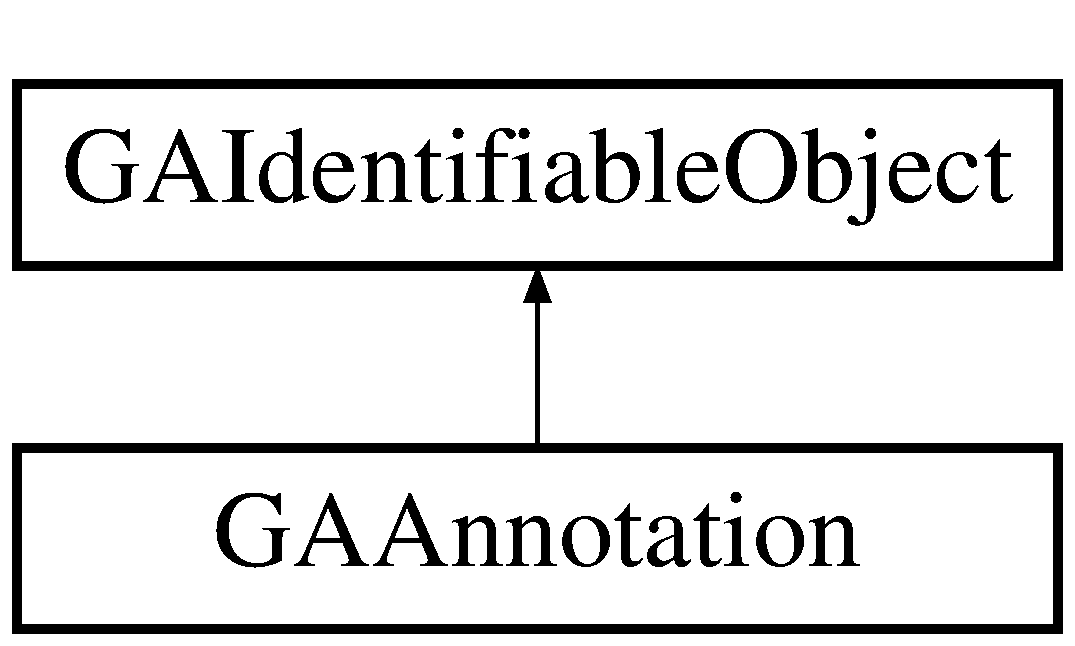
\includegraphics[height=2.000000cm]{class_g_a_annotation}
\end{center}
\end{figure}
\subsection*{Public Member Functions}
\begin{DoxyCompactItemize}
\item 
\hyperlink{class_g_a_annotation_a71e9337bdd11b745c244cb4daa370cf6}{G\+A\+Annotation} (std\+::string type)
\begin{DoxyCompactList}\small\item\em Construct a \hyperlink{class_g_a_annotation}{G\+A\+Annotation} with a type. \end{DoxyCompactList}\item 
\hyperlink{class_g_a_annotation_aa901f786bad351fe2bf19c734e6c3c92}{G\+A\+Annotation} (std\+::string id, std\+::string type)
\begin{DoxyCompactList}\small\item\em Construct a \hyperlink{class_g_a_annotation}{G\+A\+Annotation} with a persistence ID and type. \end{DoxyCompactList}\item 
\hyperlink{class_g_a_annotation_ae254750729165778f74a3d0313305eae}{G\+A\+Annotation} (std\+::string id, std\+::string type, std\+::string title)
\begin{DoxyCompactList}\small\item\em Construct a \hyperlink{class_g_a_annotation}{G\+A\+Annotation} with a persistence ID, type, and title. \end{DoxyCompactList}\item 
virtual \hyperlink{class_g_a_annotation_a68dbc2ee292a52692c33edd0b671544a}{$\sim$\+G\+A\+Annotation} ()
\begin{DoxyCompactList}\small\item\em Deconstruct the \hyperlink{class_g_a_annotation}{G\+A\+Annotation}. \end{DoxyCompactList}\item 
std\+::string \hyperlink{class_g_a_annotation_a6a5e4d1a8273090181ef60cbe06bf7c1}{get\+\_\+type} ()
\begin{DoxyCompactList}\small\item\em Get the type. \end{DoxyCompactList}\item 
void \hyperlink{class_g_a_annotation_a89552ebe856f6a6c0844e9d67237df45}{set\+\_\+type} (std\+::string type)
\begin{DoxyCompactList}\small\item\em Set the type. \end{DoxyCompactList}\item 
std\+::string \hyperlink{class_g_a_annotation_ace301a090121c29f554bc30ed5a58d53}{get\+\_\+title} ()
\begin{DoxyCompactList}\small\item\em Get the title. \end{DoxyCompactList}\item 
void \hyperlink{class_g_a_annotation_a651fe6a772d668356be8f185175b85e2}{set\+\_\+title} (std\+::string title)
\begin{DoxyCompactList}\small\item\em Set the title. \end{DoxyCompactList}\item 
std\+::string \hyperlink{class_g_a_annotation_a1e54b4980e080e1da0c40fe84443b650}{get\+\_\+description} ()
\begin{DoxyCompactList}\small\item\em Get the description. \end{DoxyCompactList}\item 
void \hyperlink{class_g_a_annotation_acd71dcf44798cafa6e9d90d3336beb81}{set\+\_\+description} (std\+::string description)
\begin{DoxyCompactList}\small\item\em Set the description. \end{DoxyCompactList}\item 
std\+::string \hyperlink{class_g_a_annotation_a2481b693d55c11c0066e6d708e7786e5}{get\+\_\+category} ()
\begin{DoxyCompactList}\small\item\em Get the category. \end{DoxyCompactList}\item 
void \hyperlink{class_g_a_annotation_ad8ed14e09ee68b1dfcff6afada72b438}{set\+\_\+category} (std\+::string category)
\begin{DoxyCompactList}\small\item\em Set the category. \end{DoxyCompactList}\item 
std\+::string \hyperlink{class_g_a_annotation_a4c309b06dcb5dec5445e281fe21f3fd2}{get\+\_\+location} ()
\begin{DoxyCompactList}\small\item\em Get the location. \end{DoxyCompactList}\item 
void \hyperlink{class_g_a_annotation_ac7f751a3088ec6e584c3b18d100cd83a}{set\+\_\+location} (std\+::string location)
\begin{DoxyCompactList}\small\item\em Set the location. \end{DoxyCompactList}\item 
\hyperlink{class_g_a_assignment_data}{G\+A\+Assignment\+Data} $\ast$ \hyperlink{class_g_a_annotation_aa99df6e807758f57b0ed5c836ec43f0e}{get\+\_\+assignment\+\_\+data} ()
\begin{DoxyCompactList}\small\item\em Get the assignment data object. \end{DoxyCompactList}\item 
void \hyperlink{class_g_a_annotation_a6dfc89a54027eefa6d3f7928faf22593}{set\+\_\+assignment\+\_\+data} (\hyperlink{class_g_a_assignment_data}{G\+A\+Assignment\+Data} $\ast$data)
\begin{DoxyCompactList}\small\item\em Set the assignment data object. \end{DoxyCompactList}\item 
bool \hyperlink{class_g_a_annotation_ad836d6b85aa860864ccc2e8afefd78cd}{save\+\_\+to} (\hyperlink{class_database_table}{Database\+Table} $\ast$table)
\begin{DoxyCompactList}\small\item\em Save the annotation to a table. \end{DoxyCompactList}\end{DoxyCompactItemize}
\subsection*{Static Public Member Functions}
\begin{DoxyCompactItemize}
\item 
static std\+::vector$<$ \hyperlink{class_g_a_annotation}{G\+A\+Annotation} $\ast$ $>$ \hyperlink{class_g_a_annotation_acbf5c9a4f95f75d7a7cf7cc6f43e00b5}{load\+\_\+from} (\hyperlink{class_database_table}{Database\+Table} $\ast$table, \hyperlink{class_g_a_assignment_data}{G\+A\+Assignment\+Data} $\ast$data)
\begin{DoxyCompactList}\small\item\em Load the annotations for an assignment data object from a table. \end{DoxyCompactList}\end{DoxyCompactItemize}


\subsection{Constructor \& Destructor Documentation}
\mbox{\Hypertarget{class_g_a_annotation_a71e9337bdd11b745c244cb4daa370cf6}\label{class_g_a_annotation_a71e9337bdd11b745c244cb4daa370cf6}} 
\index{G\+A\+Annotation@{G\+A\+Annotation}!G\+A\+Annotation@{G\+A\+Annotation}}
\index{G\+A\+Annotation@{G\+A\+Annotation}!G\+A\+Annotation@{G\+A\+Annotation}}
\subsubsection{\texorpdfstring{G\+A\+Annotation()}{GAAnnotation()}\hspace{0.1cm}{\footnotesize\ttfamily [1/3]}}
{\footnotesize\ttfamily G\+A\+Annotation\+::\+G\+A\+Annotation (\begin{DoxyParamCaption}\item[{std\+::string}]{type }\end{DoxyParamCaption})}



Construct a \hyperlink{class_g_a_annotation}{G\+A\+Annotation} with a type. 


\begin{DoxyParams}{Parameters}
{\em type} & The type \\
\hline
\end{DoxyParams}
\mbox{\Hypertarget{class_g_a_annotation_aa901f786bad351fe2bf19c734e6c3c92}\label{class_g_a_annotation_aa901f786bad351fe2bf19c734e6c3c92}} 
\index{G\+A\+Annotation@{G\+A\+Annotation}!G\+A\+Annotation@{G\+A\+Annotation}}
\index{G\+A\+Annotation@{G\+A\+Annotation}!G\+A\+Annotation@{G\+A\+Annotation}}
\subsubsection{\texorpdfstring{G\+A\+Annotation()}{GAAnnotation()}\hspace{0.1cm}{\footnotesize\ttfamily [2/3]}}
{\footnotesize\ttfamily G\+A\+Annotation\+::\+G\+A\+Annotation (\begin{DoxyParamCaption}\item[{std\+::string}]{id,  }\item[{std\+::string}]{type }\end{DoxyParamCaption})}



Construct a \hyperlink{class_g_a_annotation}{G\+A\+Annotation} with a persistence ID and type. 


\begin{DoxyParams}{Parameters}
{\em id} & The persistence ID \\
\hline
{\em type} & The type \\
\hline
\end{DoxyParams}
\mbox{\Hypertarget{class_g_a_annotation_ae254750729165778f74a3d0313305eae}\label{class_g_a_annotation_ae254750729165778f74a3d0313305eae}} 
\index{G\+A\+Annotation@{G\+A\+Annotation}!G\+A\+Annotation@{G\+A\+Annotation}}
\index{G\+A\+Annotation@{G\+A\+Annotation}!G\+A\+Annotation@{G\+A\+Annotation}}
\subsubsection{\texorpdfstring{G\+A\+Annotation()}{GAAnnotation()}\hspace{0.1cm}{\footnotesize\ttfamily [3/3]}}
{\footnotesize\ttfamily G\+A\+Annotation\+::\+G\+A\+Annotation (\begin{DoxyParamCaption}\item[{std\+::string}]{id,  }\item[{std\+::string}]{type,  }\item[{std\+::string}]{title }\end{DoxyParamCaption})}



Construct a \hyperlink{class_g_a_annotation}{G\+A\+Annotation} with a persistence ID, type, and title. 


\begin{DoxyParams}{Parameters}
{\em id} & The persistence ID \\
\hline
{\em type} & The type \\
\hline
{\em title} & The title \\
\hline
\end{DoxyParams}
\mbox{\Hypertarget{class_g_a_annotation_a68dbc2ee292a52692c33edd0b671544a}\label{class_g_a_annotation_a68dbc2ee292a52692c33edd0b671544a}} 
\index{G\+A\+Annotation@{G\+A\+Annotation}!````~G\+A\+Annotation@{$\sim$\+G\+A\+Annotation}}
\index{````~G\+A\+Annotation@{$\sim$\+G\+A\+Annotation}!G\+A\+Annotation@{G\+A\+Annotation}}
\subsubsection{\texorpdfstring{$\sim$\+G\+A\+Annotation()}{~GAAnnotation()}}
{\footnotesize\ttfamily G\+A\+Annotation\+::$\sim$\+G\+A\+Annotation (\begin{DoxyParamCaption}{ }\end{DoxyParamCaption})\hspace{0.3cm}{\ttfamily [virtual]}}



Deconstruct the \hyperlink{class_g_a_annotation}{G\+A\+Annotation}. 

Nothing currently happens here 

\subsection{Member Function Documentation}
\mbox{\Hypertarget{class_g_a_annotation_aa99df6e807758f57b0ed5c836ec43f0e}\label{class_g_a_annotation_aa99df6e807758f57b0ed5c836ec43f0e}} 
\index{G\+A\+Annotation@{G\+A\+Annotation}!get\+\_\+assignment\+\_\+data@{get\+\_\+assignment\+\_\+data}}
\index{get\+\_\+assignment\+\_\+data@{get\+\_\+assignment\+\_\+data}!G\+A\+Annotation@{G\+A\+Annotation}}
\subsubsection{\texorpdfstring{get\+\_\+assignment\+\_\+data()}{get\_assignment\_data()}}
{\footnotesize\ttfamily \hyperlink{class_g_a_assignment_data}{G\+A\+Assignment\+Data} $\ast$ G\+A\+Annotation\+::get\+\_\+assignment\+\_\+data (\begin{DoxyParamCaption}{ }\end{DoxyParamCaption})}



Get the assignment data object. 

\begin{DoxyReturn}{Returns}
The assignment data object 
\end{DoxyReturn}
\mbox{\Hypertarget{class_g_a_annotation_a2481b693d55c11c0066e6d708e7786e5}\label{class_g_a_annotation_a2481b693d55c11c0066e6d708e7786e5}} 
\index{G\+A\+Annotation@{G\+A\+Annotation}!get\+\_\+category@{get\+\_\+category}}
\index{get\+\_\+category@{get\+\_\+category}!G\+A\+Annotation@{G\+A\+Annotation}}
\subsubsection{\texorpdfstring{get\+\_\+category()}{get\_category()}}
{\footnotesize\ttfamily std\+::string G\+A\+Annotation\+::get\+\_\+category (\begin{DoxyParamCaption}{ }\end{DoxyParamCaption})}



Get the category. 

\begin{DoxyReturn}{Returns}
The category 
\end{DoxyReturn}
\mbox{\Hypertarget{class_g_a_annotation_a1e54b4980e080e1da0c40fe84443b650}\label{class_g_a_annotation_a1e54b4980e080e1da0c40fe84443b650}} 
\index{G\+A\+Annotation@{G\+A\+Annotation}!get\+\_\+description@{get\+\_\+description}}
\index{get\+\_\+description@{get\+\_\+description}!G\+A\+Annotation@{G\+A\+Annotation}}
\subsubsection{\texorpdfstring{get\+\_\+description()}{get\_description()}}
{\footnotesize\ttfamily std\+::string G\+A\+Annotation\+::get\+\_\+description (\begin{DoxyParamCaption}{ }\end{DoxyParamCaption})}



Get the description. 

\begin{DoxyReturn}{Returns}
The description 
\end{DoxyReturn}
\mbox{\Hypertarget{class_g_a_annotation_a4c309b06dcb5dec5445e281fe21f3fd2}\label{class_g_a_annotation_a4c309b06dcb5dec5445e281fe21f3fd2}} 
\index{G\+A\+Annotation@{G\+A\+Annotation}!get\+\_\+location@{get\+\_\+location}}
\index{get\+\_\+location@{get\+\_\+location}!G\+A\+Annotation@{G\+A\+Annotation}}
\subsubsection{\texorpdfstring{get\+\_\+location()}{get\_location()}}
{\footnotesize\ttfamily std\+::string G\+A\+Annotation\+::get\+\_\+location (\begin{DoxyParamCaption}{ }\end{DoxyParamCaption})}



Get the location. 

\begin{DoxyReturn}{Returns}
The location 
\end{DoxyReturn}
\mbox{\Hypertarget{class_g_a_annotation_ace301a090121c29f554bc30ed5a58d53}\label{class_g_a_annotation_ace301a090121c29f554bc30ed5a58d53}} 
\index{G\+A\+Annotation@{G\+A\+Annotation}!get\+\_\+title@{get\+\_\+title}}
\index{get\+\_\+title@{get\+\_\+title}!G\+A\+Annotation@{G\+A\+Annotation}}
\subsubsection{\texorpdfstring{get\+\_\+title()}{get\_title()}}
{\footnotesize\ttfamily std\+::string G\+A\+Annotation\+::get\+\_\+title (\begin{DoxyParamCaption}{ }\end{DoxyParamCaption})}



Get the title. 

\begin{DoxyReturn}{Returns}
The title 
\end{DoxyReturn}
\mbox{\Hypertarget{class_g_a_annotation_a6a5e4d1a8273090181ef60cbe06bf7c1}\label{class_g_a_annotation_a6a5e4d1a8273090181ef60cbe06bf7c1}} 
\index{G\+A\+Annotation@{G\+A\+Annotation}!get\+\_\+type@{get\+\_\+type}}
\index{get\+\_\+type@{get\+\_\+type}!G\+A\+Annotation@{G\+A\+Annotation}}
\subsubsection{\texorpdfstring{get\+\_\+type()}{get\_type()}}
{\footnotesize\ttfamily std\+::string G\+A\+Annotation\+::get\+\_\+type (\begin{DoxyParamCaption}{ }\end{DoxyParamCaption})}



Get the type. 

\begin{DoxyReturn}{Returns}
The type 
\end{DoxyReturn}
\mbox{\Hypertarget{class_g_a_annotation_acbf5c9a4f95f75d7a7cf7cc6f43e00b5}\label{class_g_a_annotation_acbf5c9a4f95f75d7a7cf7cc6f43e00b5}} 
\index{G\+A\+Annotation@{G\+A\+Annotation}!load\+\_\+from@{load\+\_\+from}}
\index{load\+\_\+from@{load\+\_\+from}!G\+A\+Annotation@{G\+A\+Annotation}}
\subsubsection{\texorpdfstring{load\+\_\+from()}{load\_from()}}
{\footnotesize\ttfamily std\+::vector$<$ \hyperlink{class_g_a_annotation}{G\+A\+Annotation} $\ast$ $>$ G\+A\+Annotation\+::load\+\_\+from (\begin{DoxyParamCaption}\item[{\hyperlink{class_database_table}{Database\+Table} $\ast$}]{table,  }\item[{\hyperlink{class_g_a_assignment_data}{G\+A\+Assignment\+Data} $\ast$}]{data }\end{DoxyParamCaption})\hspace{0.3cm}{\ttfamily [static]}}



Load the annotations for an assignment data object from a table. 


\begin{DoxyParams}{Parameters}
{\em table} & The table \\
\hline
{\em data} & The assignment data object \\
\hline
\end{DoxyParams}
\begin{DoxyReturn}{Returns}
The vector of annotations 
\end{DoxyReturn}
\mbox{\Hypertarget{class_g_a_annotation_ad836d6b85aa860864ccc2e8afefd78cd}\label{class_g_a_annotation_ad836d6b85aa860864ccc2e8afefd78cd}} 
\index{G\+A\+Annotation@{G\+A\+Annotation}!save\+\_\+to@{save\+\_\+to}}
\index{save\+\_\+to@{save\+\_\+to}!G\+A\+Annotation@{G\+A\+Annotation}}
\subsubsection{\texorpdfstring{save\+\_\+to()}{save\_to()}}
{\footnotesize\ttfamily bool G\+A\+Annotation\+::save\+\_\+to (\begin{DoxyParamCaption}\item[{\hyperlink{class_database_table}{Database\+Table} $\ast$}]{table }\end{DoxyParamCaption})}



Save the annotation to a table. 


\begin{DoxyParams}{Parameters}
{\em table} & The table \\
\hline
\end{DoxyParams}
\begin{DoxyReturn}{Returns}
Whether the insert was successful 
\end{DoxyReturn}
\mbox{\Hypertarget{class_g_a_annotation_a6dfc89a54027eefa6d3f7928faf22593}\label{class_g_a_annotation_a6dfc89a54027eefa6d3f7928faf22593}} 
\index{G\+A\+Annotation@{G\+A\+Annotation}!set\+\_\+assignment\+\_\+data@{set\+\_\+assignment\+\_\+data}}
\index{set\+\_\+assignment\+\_\+data@{set\+\_\+assignment\+\_\+data}!G\+A\+Annotation@{G\+A\+Annotation}}
\subsubsection{\texorpdfstring{set\+\_\+assignment\+\_\+data()}{set\_assignment\_data()}}
{\footnotesize\ttfamily void G\+A\+Annotation\+::set\+\_\+assignment\+\_\+data (\begin{DoxyParamCaption}\item[{\hyperlink{class_g_a_assignment_data}{G\+A\+Assignment\+Data} $\ast$}]{data }\end{DoxyParamCaption})}



Set the assignment data object. 


\begin{DoxyParams}{Parameters}
{\em data} & The assignment data object \\
\hline
\end{DoxyParams}
\mbox{\Hypertarget{class_g_a_annotation_ad8ed14e09ee68b1dfcff6afada72b438}\label{class_g_a_annotation_ad8ed14e09ee68b1dfcff6afada72b438}} 
\index{G\+A\+Annotation@{G\+A\+Annotation}!set\+\_\+category@{set\+\_\+category}}
\index{set\+\_\+category@{set\+\_\+category}!G\+A\+Annotation@{G\+A\+Annotation}}
\subsubsection{\texorpdfstring{set\+\_\+category()}{set\_category()}}
{\footnotesize\ttfamily void G\+A\+Annotation\+::set\+\_\+category (\begin{DoxyParamCaption}\item[{std\+::string}]{category }\end{DoxyParamCaption})}



Set the category. 


\begin{DoxyParams}{Parameters}
{\em category} & The category \\
\hline
\end{DoxyParams}
\mbox{\Hypertarget{class_g_a_annotation_acd71dcf44798cafa6e9d90d3336beb81}\label{class_g_a_annotation_acd71dcf44798cafa6e9d90d3336beb81}} 
\index{G\+A\+Annotation@{G\+A\+Annotation}!set\+\_\+description@{set\+\_\+description}}
\index{set\+\_\+description@{set\+\_\+description}!G\+A\+Annotation@{G\+A\+Annotation}}
\subsubsection{\texorpdfstring{set\+\_\+description()}{set\_description()}}
{\footnotesize\ttfamily void G\+A\+Annotation\+::set\+\_\+description (\begin{DoxyParamCaption}\item[{std\+::string}]{description }\end{DoxyParamCaption})}



Set the description. 


\begin{DoxyParams}{Parameters}
{\em description} & The description \\
\hline
\end{DoxyParams}
\mbox{\Hypertarget{class_g_a_annotation_ac7f751a3088ec6e584c3b18d100cd83a}\label{class_g_a_annotation_ac7f751a3088ec6e584c3b18d100cd83a}} 
\index{G\+A\+Annotation@{G\+A\+Annotation}!set\+\_\+location@{set\+\_\+location}}
\index{set\+\_\+location@{set\+\_\+location}!G\+A\+Annotation@{G\+A\+Annotation}}
\subsubsection{\texorpdfstring{set\+\_\+location()}{set\_location()}}
{\footnotesize\ttfamily void G\+A\+Annotation\+::set\+\_\+location (\begin{DoxyParamCaption}\item[{std\+::string}]{location }\end{DoxyParamCaption})}



Set the location. 


\begin{DoxyParams}{Parameters}
{\em location} & The location \\
\hline
\end{DoxyParams}
\mbox{\Hypertarget{class_g_a_annotation_a651fe6a772d668356be8f185175b85e2}\label{class_g_a_annotation_a651fe6a772d668356be8f185175b85e2}} 
\index{G\+A\+Annotation@{G\+A\+Annotation}!set\+\_\+title@{set\+\_\+title}}
\index{set\+\_\+title@{set\+\_\+title}!G\+A\+Annotation@{G\+A\+Annotation}}
\subsubsection{\texorpdfstring{set\+\_\+title()}{set\_title()}}
{\footnotesize\ttfamily void G\+A\+Annotation\+::set\+\_\+title (\begin{DoxyParamCaption}\item[{std\+::string}]{title }\end{DoxyParamCaption})}



Set the title. 


\begin{DoxyParams}{Parameters}
{\em title} & The title \\
\hline
\end{DoxyParams}
\mbox{\Hypertarget{class_g_a_annotation_a89552ebe856f6a6c0844e9d67237df45}\label{class_g_a_annotation_a89552ebe856f6a6c0844e9d67237df45}} 
\index{G\+A\+Annotation@{G\+A\+Annotation}!set\+\_\+type@{set\+\_\+type}}
\index{set\+\_\+type@{set\+\_\+type}!G\+A\+Annotation@{G\+A\+Annotation}}
\subsubsection{\texorpdfstring{set\+\_\+type()}{set\_type()}}
{\footnotesize\ttfamily void G\+A\+Annotation\+::set\+\_\+type (\begin{DoxyParamCaption}\item[{std\+::string}]{type }\end{DoxyParamCaption})}



Set the type. 


\begin{DoxyParams}{Parameters}
{\em type} & The type \\
\hline
\end{DoxyParams}


The documentation for this class was generated from the following files\+:\begin{DoxyCompactItemize}
\item 
grading-\/assistant/gadata/gaannotation.\+h\item 
grading-\/assistant/gadata/gaannotation.\+cpp\end{DoxyCompactItemize}

\hypertarget{class_g_a_assignment}{}\section{G\+A\+Assignment Class Reference}
\label{class_g_a_assignment}\index{G\+A\+Assignment@{G\+A\+Assignment}}
Inheritance diagram for G\+A\+Assignment\+:\begin{figure}[H]
\begin{center}
\leavevmode
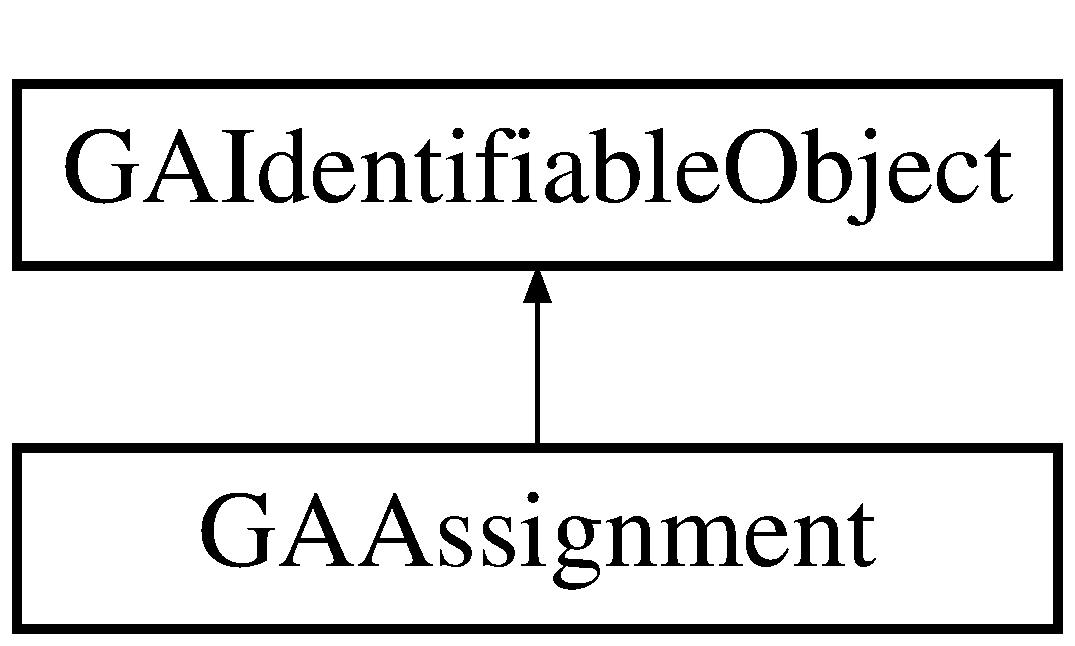
\includegraphics[height=2.000000cm]{class_g_a_assignment}
\end{center}
\end{figure}
\subsection*{Public Member Functions}
\begin{DoxyCompactItemize}
\item 
virtual \hyperlink{class_g_a_assignment_a09ccbb9ff47203cf98fce42fe934e4d2}{$\sim$\+G\+A\+Assignment} ()
\begin{DoxyCompactList}\small\item\em Deconstruct the \hyperlink{class_g_a_assignment}{G\+A\+Assignment}. \end{DoxyCompactList}\item 
std\+::string \hyperlink{class_g_a_assignment_afd2ee339549f674108e1d0cb9996c1fe}{get\+\_\+title} ()
\begin{DoxyCompactList}\small\item\em Get the title. \end{DoxyCompactList}\item 
void \hyperlink{class_g_a_assignment_ac5463bd1ed519444c85a8b4946b22e27}{set\+\_\+title} (std\+::string title)
\begin{DoxyCompactList}\small\item\em Set the title. \end{DoxyCompactList}\item 
std\+::string \hyperlink{class_g_a_assignment_aa79940e35e148a0784b70efc33f93da4}{get\+\_\+description} ()
\begin{DoxyCompactList}\small\item\em Get the description. \end{DoxyCompactList}\item 
void \hyperlink{class_g_a_assignment_ae1d657cde83c753067e77347141b49c4}{set\+\_\+description} (std\+::string description)
\begin{DoxyCompactList}\small\item\em Set the description. \end{DoxyCompactList}\item 
\hyperlink{class_g_a_class}{G\+A\+Class} $\ast$ \hyperlink{class_g_a_assignment_ae16983396d1f57845b70f607ec44dc41}{get\+\_\+class} ()
\begin{DoxyCompactList}\small\item\em Get the class this assignment is in. \end{DoxyCompactList}\item 
void \hyperlink{class_g_a_assignment_a5e54b228743afce1120b6aee837b06c0}{set\+\_\+class} (\hyperlink{class_g_a_class}{G\+A\+Class} $\ast$class\+\_\+)
\begin{DoxyCompactList}\small\item\em Set the class. \end{DoxyCompactList}\item 
bool \hyperlink{class_g_a_assignment_a2481b0469431c06bf4d28f588e3c8cf4}{save\+\_\+to} (\hyperlink{class_database_table}{Database\+Table} $\ast$table)
\begin{DoxyCompactList}\small\item\em Save this assignment to a table. \end{DoxyCompactList}\end{DoxyCompactItemize}
\subsection*{Static Public Member Functions}
\begin{DoxyCompactItemize}
\item 
static std\+::vector$<$ \hyperlink{class_g_a_assignment}{G\+A\+Assignment} $\ast$ $>$ \hyperlink{class_g_a_assignment_a167d821c1311025490e4bbbbac6d8ad4}{load\+\_\+from} (\hyperlink{class_database_table}{Database\+Table} $\ast$table, \hyperlink{class_g_a_class}{G\+A\+Class} $\ast$class\+\_\+)
\begin{DoxyCompactList}\small\item\em Load assignments from a table which are in a certain class. \end{DoxyCompactList}\end{DoxyCompactItemize}


\subsection{Constructor \& Destructor Documentation}
\mbox{\Hypertarget{class_g_a_assignment_a09ccbb9ff47203cf98fce42fe934e4d2}\label{class_g_a_assignment_a09ccbb9ff47203cf98fce42fe934e4d2}} 
\index{G\+A\+Assignment@{G\+A\+Assignment}!````~G\+A\+Assignment@{$\sim$\+G\+A\+Assignment}}
\index{````~G\+A\+Assignment@{$\sim$\+G\+A\+Assignment}!G\+A\+Assignment@{G\+A\+Assignment}}
\subsubsection{\texorpdfstring{$\sim$\+G\+A\+Assignment()}{~GAAssignment()}}
{\footnotesize\ttfamily G\+A\+Assignment\+::$\sim$\+G\+A\+Assignment (\begin{DoxyParamCaption}{ }\end{DoxyParamCaption})\hspace{0.3cm}{\ttfamily [virtual]}}



Deconstruct the \hyperlink{class_g_a_assignment}{G\+A\+Assignment}. 

Currently does nothing 

\subsection{Member Function Documentation}
\mbox{\Hypertarget{class_g_a_assignment_ae16983396d1f57845b70f607ec44dc41}\label{class_g_a_assignment_ae16983396d1f57845b70f607ec44dc41}} 
\index{G\+A\+Assignment@{G\+A\+Assignment}!get\+\_\+class@{get\+\_\+class}}
\index{get\+\_\+class@{get\+\_\+class}!G\+A\+Assignment@{G\+A\+Assignment}}
\subsubsection{\texorpdfstring{get\+\_\+class()}{get\_class()}}
{\footnotesize\ttfamily \hyperlink{class_g_a_class}{G\+A\+Class} $\ast$ G\+A\+Assignment\+::get\+\_\+class (\begin{DoxyParamCaption}{ }\end{DoxyParamCaption})}



Get the class this assignment is in. 

\begin{DoxyReturn}{Returns}
The class 
\end{DoxyReturn}
\mbox{\Hypertarget{class_g_a_assignment_aa79940e35e148a0784b70efc33f93da4}\label{class_g_a_assignment_aa79940e35e148a0784b70efc33f93da4}} 
\index{G\+A\+Assignment@{G\+A\+Assignment}!get\+\_\+description@{get\+\_\+description}}
\index{get\+\_\+description@{get\+\_\+description}!G\+A\+Assignment@{G\+A\+Assignment}}
\subsubsection{\texorpdfstring{get\+\_\+description()}{get\_description()}}
{\footnotesize\ttfamily std\+::string G\+A\+Assignment\+::get\+\_\+description (\begin{DoxyParamCaption}{ }\end{DoxyParamCaption})}



Get the description. 

\begin{DoxyReturn}{Returns}
The description 
\end{DoxyReturn}
\mbox{\Hypertarget{class_g_a_assignment_afd2ee339549f674108e1d0cb9996c1fe}\label{class_g_a_assignment_afd2ee339549f674108e1d0cb9996c1fe}} 
\index{G\+A\+Assignment@{G\+A\+Assignment}!get\+\_\+title@{get\+\_\+title}}
\index{get\+\_\+title@{get\+\_\+title}!G\+A\+Assignment@{G\+A\+Assignment}}
\subsubsection{\texorpdfstring{get\+\_\+title()}{get\_title()}}
{\footnotesize\ttfamily std\+::string G\+A\+Assignment\+::get\+\_\+title (\begin{DoxyParamCaption}{ }\end{DoxyParamCaption})}



Get the title. 

\begin{DoxyReturn}{Returns}
The title 
\end{DoxyReturn}
\mbox{\Hypertarget{class_g_a_assignment_a167d821c1311025490e4bbbbac6d8ad4}\label{class_g_a_assignment_a167d821c1311025490e4bbbbac6d8ad4}} 
\index{G\+A\+Assignment@{G\+A\+Assignment}!load\+\_\+from@{load\+\_\+from}}
\index{load\+\_\+from@{load\+\_\+from}!G\+A\+Assignment@{G\+A\+Assignment}}
\subsubsection{\texorpdfstring{load\+\_\+from()}{load\_from()}}
{\footnotesize\ttfamily std\+::vector$<$ \hyperlink{class_g_a_assignment}{G\+A\+Assignment} $\ast$ $>$ G\+A\+Assignment\+::load\+\_\+from (\begin{DoxyParamCaption}\item[{\hyperlink{class_database_table}{Database\+Table} $\ast$}]{table,  }\item[{\hyperlink{class_g_a_class}{G\+A\+Class} $\ast$}]{class\+\_\+ }\end{DoxyParamCaption})\hspace{0.3cm}{\ttfamily [static]}}



Load assignments from a table which are in a certain class. 


\begin{DoxyParams}{Parameters}
{\em table} & The table \\
\hline
{\em class\+\_\+} & The class \\
\hline
\end{DoxyParams}
\begin{DoxyReturn}{Returns}
The list of assignments 
\end{DoxyReturn}
\mbox{\Hypertarget{class_g_a_assignment_a2481b0469431c06bf4d28f588e3c8cf4}\label{class_g_a_assignment_a2481b0469431c06bf4d28f588e3c8cf4}} 
\index{G\+A\+Assignment@{G\+A\+Assignment}!save\+\_\+to@{save\+\_\+to}}
\index{save\+\_\+to@{save\+\_\+to}!G\+A\+Assignment@{G\+A\+Assignment}}
\subsubsection{\texorpdfstring{save\+\_\+to()}{save\_to()}}
{\footnotesize\ttfamily bool G\+A\+Assignment\+::save\+\_\+to (\begin{DoxyParamCaption}\item[{\hyperlink{class_database_table}{Database\+Table} $\ast$}]{table }\end{DoxyParamCaption})}



Save this assignment to a table. 


\begin{DoxyParams}{Parameters}
{\em table} & The table \\
\hline
\end{DoxyParams}
\begin{DoxyReturn}{Returns}
The table 
\end{DoxyReturn}
\mbox{\Hypertarget{class_g_a_assignment_a5e54b228743afce1120b6aee837b06c0}\label{class_g_a_assignment_a5e54b228743afce1120b6aee837b06c0}} 
\index{G\+A\+Assignment@{G\+A\+Assignment}!set\+\_\+class@{set\+\_\+class}}
\index{set\+\_\+class@{set\+\_\+class}!G\+A\+Assignment@{G\+A\+Assignment}}
\subsubsection{\texorpdfstring{set\+\_\+class()}{set\_class()}}
{\footnotesize\ttfamily void G\+A\+Assignment\+::set\+\_\+class (\begin{DoxyParamCaption}\item[{\hyperlink{class_g_a_class}{G\+A\+Class} $\ast$}]{class\+\_\+ }\end{DoxyParamCaption})}



Set the class. 

Do not call this method directly, instead use the \hyperlink{class_g_a_class}{G\+A\+Class} methods to add it.


\begin{DoxyParams}{Parameters}
{\em class\+\_\+} & The class \\
\hline
\end{DoxyParams}
\mbox{\Hypertarget{class_g_a_assignment_ae1d657cde83c753067e77347141b49c4}\label{class_g_a_assignment_ae1d657cde83c753067e77347141b49c4}} 
\index{G\+A\+Assignment@{G\+A\+Assignment}!set\+\_\+description@{set\+\_\+description}}
\index{set\+\_\+description@{set\+\_\+description}!G\+A\+Assignment@{G\+A\+Assignment}}
\subsubsection{\texorpdfstring{set\+\_\+description()}{set\_description()}}
{\footnotesize\ttfamily void G\+A\+Assignment\+::set\+\_\+description (\begin{DoxyParamCaption}\item[{std\+::string}]{description }\end{DoxyParamCaption})}



Set the description. 


\begin{DoxyParams}{Parameters}
{\em description} & The description \\
\hline
\end{DoxyParams}
\mbox{\Hypertarget{class_g_a_assignment_ac5463bd1ed519444c85a8b4946b22e27}\label{class_g_a_assignment_ac5463bd1ed519444c85a8b4946b22e27}} 
\index{G\+A\+Assignment@{G\+A\+Assignment}!set\+\_\+title@{set\+\_\+title}}
\index{set\+\_\+title@{set\+\_\+title}!G\+A\+Assignment@{G\+A\+Assignment}}
\subsubsection{\texorpdfstring{set\+\_\+title()}{set\_title()}}
{\footnotesize\ttfamily void G\+A\+Assignment\+::set\+\_\+title (\begin{DoxyParamCaption}\item[{std\+::string}]{title }\end{DoxyParamCaption})}



Set the title. 


\begin{DoxyParams}{Parameters}
{\em title} & The title \\
\hline
\end{DoxyParams}


The documentation for this class was generated from the following files\+:\begin{DoxyCompactItemize}
\item 
grading-\/assistant/gadata/gaassignment.\+h\item 
grading-\/assistant/gadata/gaassignment.\+cpp\end{DoxyCompactItemize}

\hypertarget{class_g_a_assignment_data}{}\section{G\+A\+Assignment\+Data Class Reference}
\label{class_g_a_assignment_data}\index{G\+A\+Assignment\+Data@{G\+A\+Assignment\+Data}}
Inheritance diagram for G\+A\+Assignment\+Data\+:\begin{figure}[H]
\begin{center}
\leavevmode
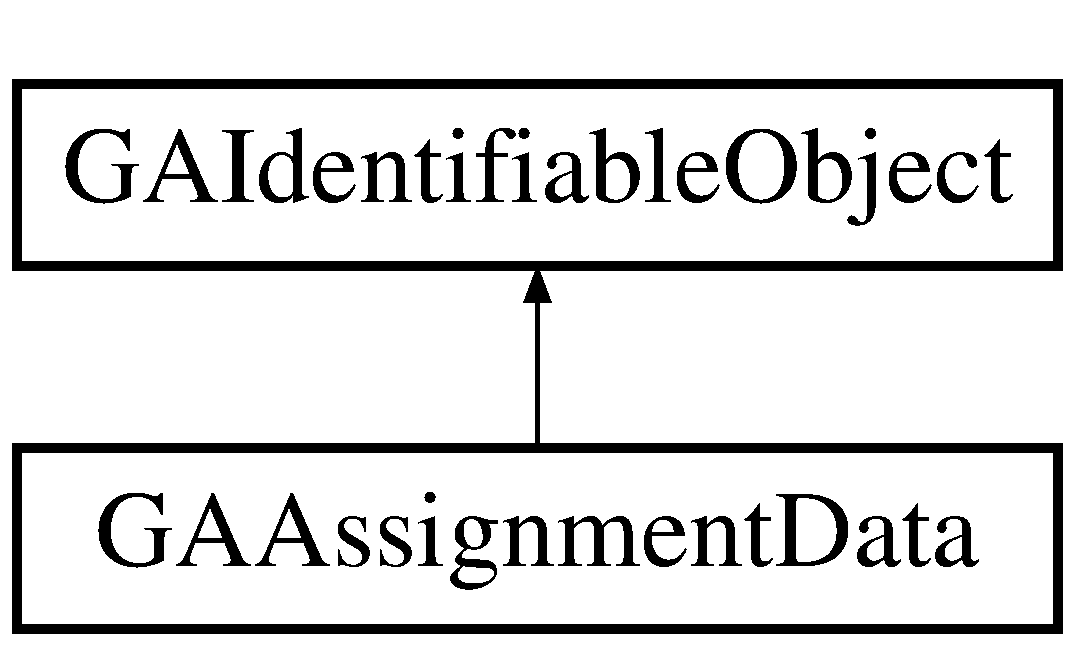
\includegraphics[height=2.000000cm]{class_g_a_assignment_data}
\end{center}
\end{figure}
\subsection*{Public Member Functions}
\begin{DoxyCompactItemize}
\item 
\mbox{\Hypertarget{class_g_a_assignment_data_a780a6615197aedd52b5949039c5dcec6}\label{class_g_a_assignment_data_a780a6615197aedd52b5949039c5dcec6}} 
\hyperlink{class_g_a_assignment}{G\+A\+Assignment} $\ast$ {\bfseries get\+\_\+assignment} ()
\item 
\mbox{\Hypertarget{class_g_a_assignment_data_ae03cdaeba3a52203d53464f680ad771b}\label{class_g_a_assignment_data_ae03cdaeba3a52203d53464f680ad771b}} 
void {\bfseries set\+\_\+assignment} (\hyperlink{class_g_a_assignment}{G\+A\+Assignment} $\ast$a)
\item 
\mbox{\Hypertarget{class_g_a_assignment_data_a74258a84379424b3e3f34775651426bf}\label{class_g_a_assignment_data_a74258a84379424b3e3f34775651426bf}} 
\hyperlink{class_g_a_student}{G\+A\+Student} $\ast$ {\bfseries get\+\_\+student} ()
\item 
\mbox{\Hypertarget{class_g_a_assignment_data_adfad0e5c33b77ef03fd654b04d1354d7}\label{class_g_a_assignment_data_adfad0e5c33b77ef03fd654b04d1354d7}} 
void {\bfseries set\+\_\+student} (\hyperlink{class_g_a_student}{G\+A\+Student} $\ast$a)
\item 
\mbox{\Hypertarget{class_g_a_assignment_data_a04efbb8e93f6e767fd496253920521c2}\label{class_g_a_assignment_data_a04efbb8e93f6e767fd496253920521c2}} 
void {\bfseries add\+\_\+annotation} (\hyperlink{class_g_a_annotation}{G\+A\+Annotation} $\ast$a)
\item 
\mbox{\Hypertarget{class_g_a_assignment_data_a608a62cbabb5450fc8968f29f69bece0}\label{class_g_a_assignment_data_a608a62cbabb5450fc8968f29f69bece0}} 
std\+::vector$<$ \hyperlink{class_g_a_annotation}{G\+A\+Annotation} $\ast$ $>$ {\bfseries get\+\_\+comments} ()
\item 
\mbox{\Hypertarget{class_g_a_assignment_data_a8e57bebc0847439a72ef18ffe2b7d85d}\label{class_g_a_assignment_data_a8e57bebc0847439a72ef18ffe2b7d85d}} 
std\+::vector$<$ \hyperlink{class_g_a_annotation}{G\+A\+Annotation} $\ast$ $>$ {\bfseries get\+\_\+problems} ()
\item 
\mbox{\Hypertarget{class_g_a_assignment_data_a9f82e8c4ed81e51f2c4086e2748d8c04}\label{class_g_a_assignment_data_a9f82e8c4ed81e51f2c4086e2748d8c04}} 
std\+::vector$<$ \hyperlink{class_g_a_annotation}{G\+A\+Annotation} $\ast$ $>$ {\bfseries get\+\_\+extra\+\_\+credit} ()
\item 
\mbox{\Hypertarget{class_g_a_assignment_data_a92242c8196bf3f97927ecc11fa52c816}\label{class_g_a_assignment_data_a92242c8196bf3f97927ecc11fa52c816}} 
std\+::vector$<$ \hyperlink{class_g_a_annotation}{G\+A\+Annotation} $\ast$ $>$ {\bfseries get\+\_\+by\+\_\+type} (std\+::string type)
\item 
\mbox{\Hypertarget{class_g_a_assignment_data_ac64a01956680a8700dca510945e84709}\label{class_g_a_assignment_data_ac64a01956680a8700dca510945e84709}} 
std\+::vector$<$ \hyperlink{class_g_a_annotation}{G\+A\+Annotation} $\ast$ $>$ {\bfseries get\+\_\+annotations} ()
\item 
\mbox{\Hypertarget{class_g_a_assignment_data_a09c5f8e49023e513fca995ed192e6faf}\label{class_g_a_assignment_data_a09c5f8e49023e513fca995ed192e6faf}} 
bool {\bfseries save\+\_\+to} (\hyperlink{class_database_table}{Database\+Table} $\ast$table)
\end{DoxyCompactItemize}
\subsection*{Static Public Member Functions}
\begin{DoxyCompactItemize}
\item 
\mbox{\Hypertarget{class_g_a_assignment_data_a31ed802f1ef4b21bd9f47024a80bf4bd}\label{class_g_a_assignment_data_a31ed802f1ef4b21bd9f47024a80bf4bd}} 
static \hyperlink{class_g_a_assignment_data}{G\+A\+Assignment\+Data} $\ast$ {\bfseries load\+\_\+from} (\hyperlink{class_database_table}{Database\+Table} $\ast$table, \hyperlink{class_g_a_assignment}{G\+A\+Assignment} $\ast$assignment, \hyperlink{class_g_a_student}{G\+A\+Student} $\ast$student)
\end{DoxyCompactItemize}


The documentation for this class was generated from the following files\+:\begin{DoxyCompactItemize}
\item 
grading-\/assistant/gadata/gaassignmentdata.\+h\item 
grading-\/assistant/gadata/gaassignmentdata.\+cpp\end{DoxyCompactItemize}

\hypertarget{class_g_a_class}{}\section{G\+A\+Class Class Reference}
\label{class_g_a_class}\index{G\+A\+Class@{G\+A\+Class}}
Inheritance diagram for G\+A\+Class\+:\begin{figure}[H]
\begin{center}
\leavevmode
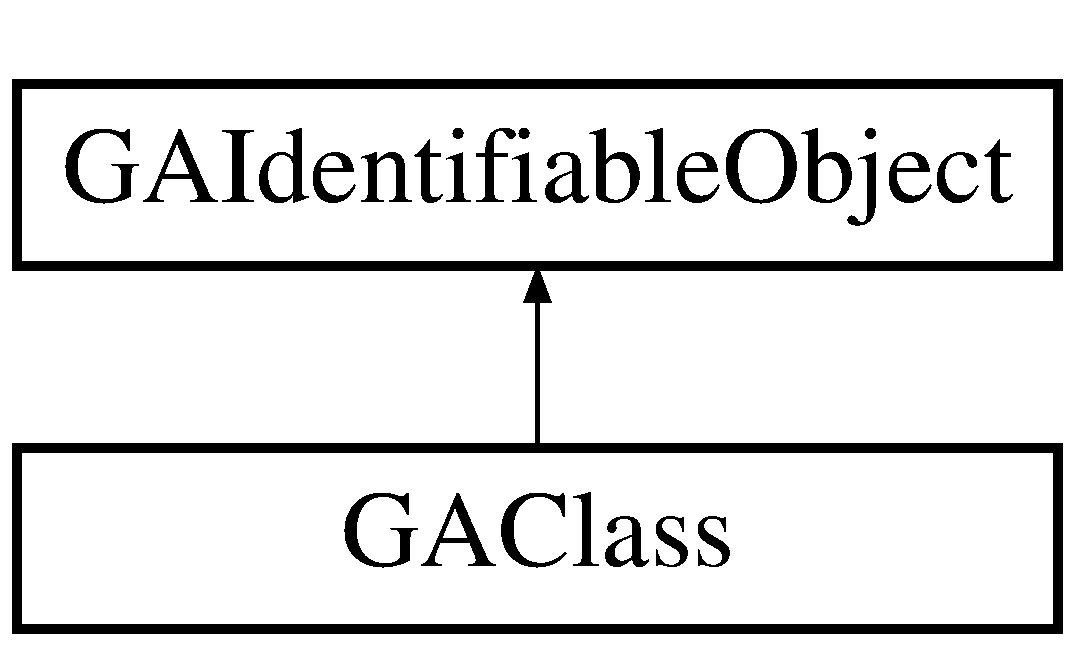
\includegraphics[height=2.000000cm]{class_g_a_class}
\end{center}
\end{figure}
\subsection*{Public Member Functions}
\begin{DoxyCompactItemize}
\item 
\mbox{\Hypertarget{class_g_a_class_ab520f3410c2112a8a9dee4f1819ae46a}\label{class_g_a_class_ab520f3410c2112a8a9dee4f1819ae46a}} 
{\bfseries G\+A\+Class} (std\+::string name)
\item 
\mbox{\Hypertarget{class_g_a_class_a945aa950aa43a22d88e800eed2a99f2f}\label{class_g_a_class_a945aa950aa43a22d88e800eed2a99f2f}} 
{\bfseries G\+A\+Class} (std\+::string id, std\+::string name)
\item 
\mbox{\Hypertarget{class_g_a_class_aa8f1809a862a8033cb2b483d5171766f}\label{class_g_a_class_aa8f1809a862a8033cb2b483d5171766f}} 
std\+::string {\bfseries get\+\_\+name} ()
\item 
\mbox{\Hypertarget{class_g_a_class_acdc31db88ea63107ebe71515adcb6d95}\label{class_g_a_class_acdc31db88ea63107ebe71515adcb6d95}} 
void {\bfseries set\+\_\+name} (std\+::string name)
\item 
\mbox{\Hypertarget{class_g_a_class_a121d237710301ee81cc112c40997dddb}\label{class_g_a_class_a121d237710301ee81cc112c40997dddb}} 
std\+::vector$<$ \hyperlink{class_g_a_student}{G\+A\+Student} $\ast$ $>$ {\bfseries get\+\_\+students} ()
\item 
\mbox{\Hypertarget{class_g_a_class_a3ac2976fe89c09df2aa3169d18c03332}\label{class_g_a_class_a3ac2976fe89c09df2aa3169d18c03332}} 
void {\bfseries add\+\_\+student} (\hyperlink{class_g_a_student}{G\+A\+Student} $\ast$student)
\item 
\mbox{\Hypertarget{class_g_a_class_acba6a56f7dd354fb2c503607d6160baf}\label{class_g_a_class_acba6a56f7dd354fb2c503607d6160baf}} 
void {\bfseries remove\+\_\+student} (\hyperlink{class_g_a_student}{G\+A\+Student} $\ast$student)
\item 
\mbox{\Hypertarget{class_g_a_class_a13ff8c6f399b1eb75b594398d39a28ff}\label{class_g_a_class_a13ff8c6f399b1eb75b594398d39a28ff}} 
std\+::vector$<$ \hyperlink{class_g_a_assignment}{G\+A\+Assignment} $\ast$ $>$ {\bfseries get\+\_\+assignments} ()
\item 
\mbox{\Hypertarget{class_g_a_class_a0e16dab0bd0e7fa2d226e2a3d9ee6454}\label{class_g_a_class_a0e16dab0bd0e7fa2d226e2a3d9ee6454}} 
void {\bfseries add\+\_\+assignment} (\hyperlink{class_g_a_assignment}{G\+A\+Assignment} $\ast$assignment)
\item 
\mbox{\Hypertarget{class_g_a_class_ad1dedccf3f22604d76a9d61f73e899fc}\label{class_g_a_class_ad1dedccf3f22604d76a9d61f73e899fc}} 
bool {\bfseries save\+\_\+to} (\hyperlink{class_database_table}{Database\+Table} $\ast$table)
\item 
\mbox{\Hypertarget{class_g_a_class_ac06d387b61bbafe7860e08f4b00148a4}\label{class_g_a_class_ac06d387b61bbafe7860e08f4b00148a4}} 
std\+::string {\bfseries to\+\_\+string} ()
\end{DoxyCompactItemize}
\subsection*{Static Public Member Functions}
\begin{DoxyCompactItemize}
\item 
\mbox{\Hypertarget{class_g_a_class_a0622a9e16a1dbecf97ec213b951e974b}\label{class_g_a_class_a0622a9e16a1dbecf97ec213b951e974b}} 
static std\+::vector$<$ \hyperlink{class_g_a_class}{G\+A\+Class} $\ast$ $>$ {\bfseries load\+\_\+from} (\hyperlink{class_database_table}{Database\+Table} $\ast$table)
\end{DoxyCompactItemize}


The documentation for this class was generated from the following files\+:\begin{DoxyCompactItemize}
\item 
grading-\/assistant/gadata/gaclass.\+h\item 
grading-\/assistant/gadata/gaclass.\+cpp\end{DoxyCompactItemize}

\hypertarget{class_g_a_identifiable_object}{}\section{G\+A\+Identifiable\+Object Class Reference}
\label{class_g_a_identifiable_object}\index{G\+A\+Identifiable\+Object@{G\+A\+Identifiable\+Object}}
Inheritance diagram for G\+A\+Identifiable\+Object\+:\begin{figure}[H]
\begin{center}
\leavevmode
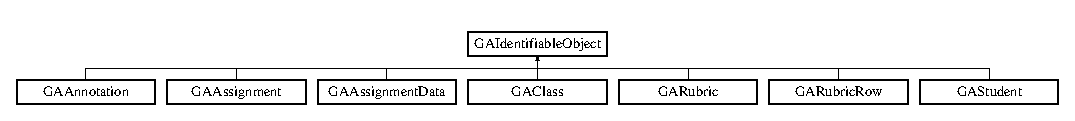
\includegraphics[height=1.176471cm]{class_g_a_identifiable_object}
\end{center}
\end{figure}
\subsection*{Public Member Functions}
\begin{DoxyCompactItemize}
\item 
\hyperlink{class_g_a_identifiable_object_a22300b23e98b09ca27b87f50cecdd1da}{G\+A\+Identifiable\+Object} ()
\begin{DoxyCompactList}\small\item\em Create with a random ID. \end{DoxyCompactList}\item 
\hyperlink{class_g_a_identifiable_object_a80ca248b066ca01681ebbc89a7f32c03}{G\+A\+Identifiable\+Object} (std\+::string id)
\begin{DoxyCompactList}\small\item\em Create a new object with a provided ID. \end{DoxyCompactList}\item 
\mbox{\Hypertarget{class_g_a_identifiable_object_ae9fef38488c8d16b03bb0cfffd600259}\label{class_g_a_identifiable_object_ae9fef38488c8d16b03bb0cfffd600259}} 
virtual \hyperlink{class_g_a_identifiable_object_ae9fef38488c8d16b03bb0cfffd600259}{$\sim$\+G\+A\+Identifiable\+Object} ()
\begin{DoxyCompactList}\small\item\em Deconstruct the G\+A\+Identiable\+Object. \end{DoxyCompactList}\item 
std\+::string \hyperlink{class_g_a_identifiable_object_afdd3c5022366b4e963c2b194f55c9400}{get\+\_\+id} ()
\begin{DoxyCompactList}\small\item\em Get the ID of the object. \end{DoxyCompactList}\item 
void \hyperlink{class_g_a_identifiable_object_a6b0a4580ef8e6e3f9b0a39fbc9d424e0}{set\+\_\+id} (std\+::string id)
\begin{DoxyCompactList}\small\item\em Set the ID of the object. \end{DoxyCompactList}\end{DoxyCompactItemize}


\subsection{Constructor \& Destructor Documentation}
\mbox{\Hypertarget{class_g_a_identifiable_object_a22300b23e98b09ca27b87f50cecdd1da}\label{class_g_a_identifiable_object_a22300b23e98b09ca27b87f50cecdd1da}} 
\index{G\+A\+Identifiable\+Object@{G\+A\+Identifiable\+Object}!G\+A\+Identifiable\+Object@{G\+A\+Identifiable\+Object}}
\index{G\+A\+Identifiable\+Object@{G\+A\+Identifiable\+Object}!G\+A\+Identifiable\+Object@{G\+A\+Identifiable\+Object}}
\subsubsection{\texorpdfstring{G\+A\+Identifiable\+Object()}{GAIdentifiableObject()}\hspace{0.1cm}{\footnotesize\ttfamily [1/2]}}
{\footnotesize\ttfamily G\+A\+Identifiable\+Object\+::\+G\+A\+Identifiable\+Object (\begin{DoxyParamCaption}{ }\end{DoxyParamCaption})}



Create with a random ID. 

If loading an object from the database, be sure to call \hyperlink{class_g_a_identifiable_object_a6b0a4580ef8e6e3f9b0a39fbc9d424e0}{set\+\_\+id(std\+::string id)} afterwards \mbox{\Hypertarget{class_g_a_identifiable_object_a80ca248b066ca01681ebbc89a7f32c03}\label{class_g_a_identifiable_object_a80ca248b066ca01681ebbc89a7f32c03}} 
\index{G\+A\+Identifiable\+Object@{G\+A\+Identifiable\+Object}!G\+A\+Identifiable\+Object@{G\+A\+Identifiable\+Object}}
\index{G\+A\+Identifiable\+Object@{G\+A\+Identifiable\+Object}!G\+A\+Identifiable\+Object@{G\+A\+Identifiable\+Object}}
\subsubsection{\texorpdfstring{G\+A\+Identifiable\+Object()}{GAIdentifiableObject()}\hspace{0.1cm}{\footnotesize\ttfamily [2/2]}}
{\footnotesize\ttfamily G\+A\+Identifiable\+Object\+::\+G\+A\+Identifiable\+Object (\begin{DoxyParamCaption}\item[{std\+::string}]{id }\end{DoxyParamCaption})}



Create a new object with a provided ID. 


\begin{DoxyParams}{Parameters}
{\em id} & The ID to use \\
\hline
\end{DoxyParams}


\subsection{Member Function Documentation}
\mbox{\Hypertarget{class_g_a_identifiable_object_afdd3c5022366b4e963c2b194f55c9400}\label{class_g_a_identifiable_object_afdd3c5022366b4e963c2b194f55c9400}} 
\index{G\+A\+Identifiable\+Object@{G\+A\+Identifiable\+Object}!get\+\_\+id@{get\+\_\+id}}
\index{get\+\_\+id@{get\+\_\+id}!G\+A\+Identifiable\+Object@{G\+A\+Identifiable\+Object}}
\subsubsection{\texorpdfstring{get\+\_\+id()}{get\_id()}}
{\footnotesize\ttfamily std\+::string G\+A\+Identifiable\+Object\+::get\+\_\+id (\begin{DoxyParamCaption}{ }\end{DoxyParamCaption})}



Get the ID of the object. 

\begin{DoxyReturn}{Returns}
The ID of the object. Will always be 38 characters 
\end{DoxyReturn}
\mbox{\Hypertarget{class_g_a_identifiable_object_a6b0a4580ef8e6e3f9b0a39fbc9d424e0}\label{class_g_a_identifiable_object_a6b0a4580ef8e6e3f9b0a39fbc9d424e0}} 
\index{G\+A\+Identifiable\+Object@{G\+A\+Identifiable\+Object}!set\+\_\+id@{set\+\_\+id}}
\index{set\+\_\+id@{set\+\_\+id}!G\+A\+Identifiable\+Object@{G\+A\+Identifiable\+Object}}
\subsubsection{\texorpdfstring{set\+\_\+id()}{set\_id()}}
{\footnotesize\ttfamily void G\+A\+Identifiable\+Object\+::set\+\_\+id (\begin{DoxyParamCaption}\item[{std\+::string}]{id }\end{DoxyParamCaption})}



Set the ID of the object. 


\begin{DoxyParams}{Parameters}
{\em id} & The new ID \\
\hline
\end{DoxyParams}


The documentation for this class was generated from the following files\+:\begin{DoxyCompactItemize}
\item 
grading-\/assistant/gadata/gaidentifiableobject.\+h\item 
grading-\/assistant/gadata/gaidentifiableobject.\+cpp\end{DoxyCompactItemize}

\hypertarget{class_g_a_rubric}{}\section{G\+A\+Rubric Class Reference}
\label{class_g_a_rubric}\index{G\+A\+Rubric@{G\+A\+Rubric}}
Inheritance diagram for G\+A\+Rubric\+:\begin{figure}[H]
\begin{center}
\leavevmode
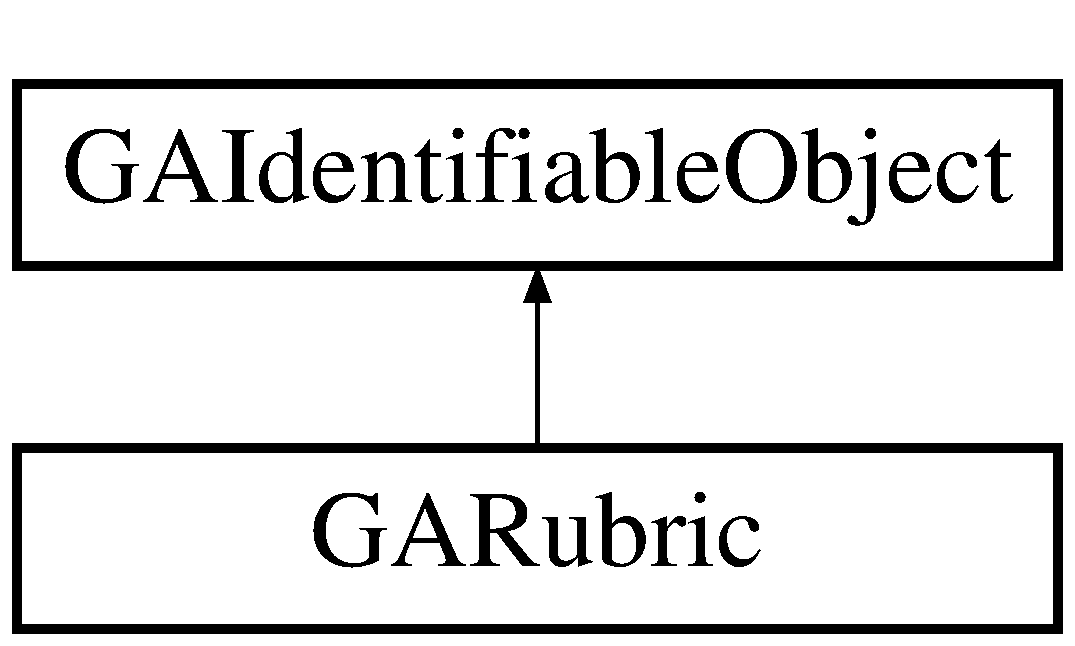
\includegraphics[height=2.000000cm]{class_g_a_rubric}
\end{center}
\end{figure}
\subsection*{Public Member Functions}
\begin{DoxyCompactItemize}
\item 
\mbox{\Hypertarget{class_g_a_rubric_a2a9233529a975bd8a26b7866f2d44cf1}\label{class_g_a_rubric_a2a9233529a975bd8a26b7866f2d44cf1}} 
{\bfseries G\+A\+Rubric} (std\+::string title, int max\+Points)
\item 
\mbox{\Hypertarget{class_g_a_rubric_a7d12ae44574c9db7fc48043321d02987}\label{class_g_a_rubric_a7d12ae44574c9db7fc48043321d02987}} 
std\+::string {\bfseries get\+\_\+title} ()
\item 
\mbox{\Hypertarget{class_g_a_rubric_a9d6eb1655668d974c094a7a5c4e0d736}\label{class_g_a_rubric_a9d6eb1655668d974c094a7a5c4e0d736}} 
void {\bfseries set\+\_\+title} (std\+::string t)
\item 
\mbox{\Hypertarget{class_g_a_rubric_a1bc73cf6dbbd107c3396d12163efa2ab}\label{class_g_a_rubric_a1bc73cf6dbbd107c3396d12163efa2ab}} 
int {\bfseries get\+\_\+max\+\_\+points} ()
\item 
\mbox{\Hypertarget{class_g_a_rubric_abcd98dc85cdbf4abe0d66503b9aaad06}\label{class_g_a_rubric_abcd98dc85cdbf4abe0d66503b9aaad06}} 
void {\bfseries set\+\_\+max\+\_\+points} (int mP)
\item 
\mbox{\Hypertarget{class_g_a_rubric_a4b2d36c27c9d45501f8e6f11c1747cf5}\label{class_g_a_rubric_a4b2d36c27c9d45501f8e6f11c1747cf5}} 
std\+::vector$<$ \hyperlink{class_g_a_rubric_row}{G\+A\+Rubric\+Row} $\ast$ $>$ {\bfseries get\+\_\+rows} ()
\item 
\mbox{\Hypertarget{class_g_a_rubric_af039f5d2ff581616a1bdb5cd7c574a00}\label{class_g_a_rubric_af039f5d2ff581616a1bdb5cd7c574a00}} 
void {\bfseries add\+\_\+row} (\hyperlink{class_g_a_rubric_row}{G\+A\+Rubric\+Row} $\ast$row)
\item 
\mbox{\Hypertarget{class_g_a_rubric_aa09ea9945e571bca75f56484c3d11711}\label{class_g_a_rubric_aa09ea9945e571bca75f56484c3d11711}} 
\hyperlink{class_g_a_rubric_row}{G\+A\+Rubric\+Row} $\ast$ {\bfseries add\+\_\+row} (std\+::string category, std\+::string description, int point\+Value)
\item 
\mbox{\Hypertarget{class_g_a_rubric_a6941a873945e03c666bd4de6fd12031e}\label{class_g_a_rubric_a6941a873945e03c666bd4de6fd12031e}} 
\hyperlink{class_g_a_rubric_row}{G\+A\+Rubric\+Row} $\ast$ {\bfseries add\+\_\+row} (std\+::string category, std\+::vector$<$ std\+::string $>$ descriptions, int point\+Value)
\item 
\mbox{\Hypertarget{class_g_a_rubric_a7fcc45b5adcc76d3ba11eb1a3189553c}\label{class_g_a_rubric_a7fcc45b5adcc76d3ba11eb1a3189553c}} 
\hyperlink{class_g_a_rubric_row}{G\+A\+Rubric\+Row} $\ast$ {\bfseries get\+\_\+ec} ()
\item 
\mbox{\Hypertarget{class_g_a_rubric_aa4b476559c0c28086da6393c74fd2a57}\label{class_g_a_rubric_aa4b476559c0c28086da6393c74fd2a57}} 
\hyperlink{class_g_a_rubric_row}{G\+A\+Rubric\+Row} $\ast$ {\bfseries set\+\_\+ec} (std\+::string category, std\+::string description, int point\+Value)
\item 
\mbox{\Hypertarget{class_g_a_rubric_a35176e486e148314b02890ed00986f9b}\label{class_g_a_rubric_a35176e486e148314b02890ed00986f9b}} 
void {\bfseries set\+\_\+ec} (\hyperlink{class_g_a_rubric_row}{G\+A\+Rubric\+Row} $\ast$row)
\item 
\mbox{\Hypertarget{class_g_a_rubric_a9999dba278704374dd8326892257c351}\label{class_g_a_rubric_a9999dba278704374dd8326892257c351}} 
bool {\bfseries save\+\_\+to} (\hyperlink{class_database_table}{Database\+Table} $\ast$table)
\end{DoxyCompactItemize}
\subsection*{Static Public Member Functions}
\begin{DoxyCompactItemize}
\item 
\mbox{\Hypertarget{class_g_a_rubric_ac7180d84cb7943e26f90bc43b9c19d03}\label{class_g_a_rubric_ac7180d84cb7943e26f90bc43b9c19d03}} 
static std\+::vector$<$ \hyperlink{class_g_a_rubric}{G\+A\+Rubric} $\ast$ $>$ {\bfseries load\+\_\+from} (\hyperlink{class_database_table}{Database\+Table} $\ast$table)
\end{DoxyCompactItemize}


The documentation for this class was generated from the following files\+:\begin{DoxyCompactItemize}
\item 
grading-\/assistant/gadata/garubric.\+h\item 
grading-\/assistant/gadata/garubric.\+cpp\end{DoxyCompactItemize}

\hypertarget{class_g_a_rubric_row}{}\section{G\+A\+Rubric\+Row Class Reference}
\label{class_g_a_rubric_row}\index{G\+A\+Rubric\+Row@{G\+A\+Rubric\+Row}}
Inheritance diagram for G\+A\+Rubric\+Row\+:\begin{figure}[H]
\begin{center}
\leavevmode
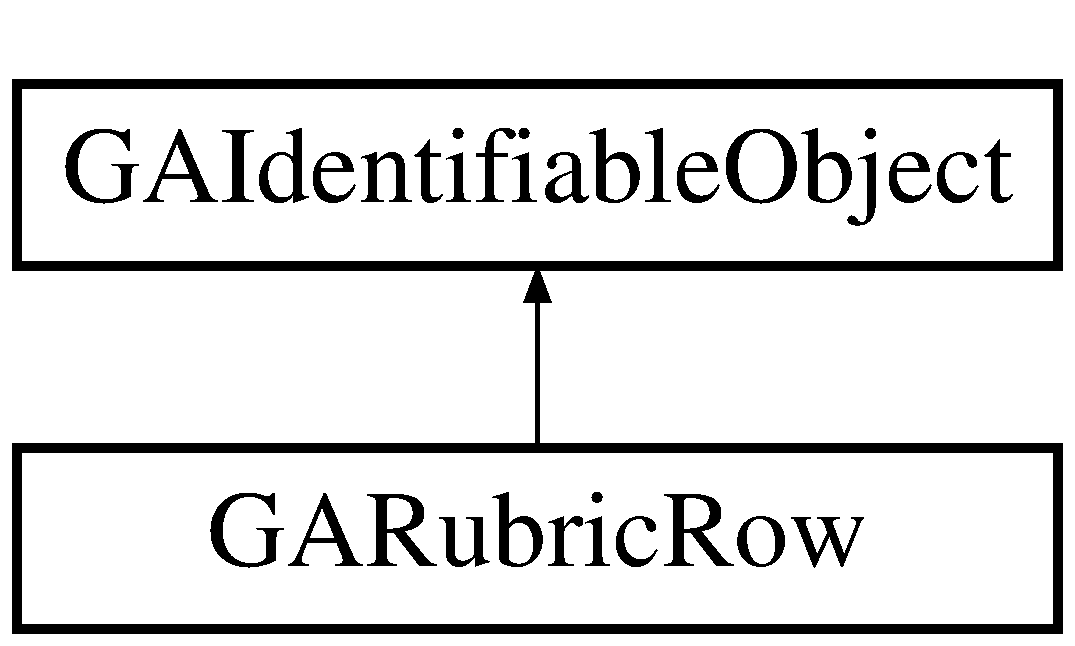
\includegraphics[height=2.000000cm]{class_g_a_rubric_row}
\end{center}
\end{figure}
\subsection*{Public Member Functions}
\begin{DoxyCompactItemize}
\item 
\mbox{\Hypertarget{class_g_a_rubric_row_ac537d4b51105cc03231b2940e8deb98a}\label{class_g_a_rubric_row_ac537d4b51105cc03231b2940e8deb98a}} 
{\bfseries G\+A\+Rubric\+Row} (std\+::string category, std\+::string description, int total\+\_\+points)
\item 
\mbox{\Hypertarget{class_g_a_rubric_row_a84bb1a3b310e8d286cccc236ef777233}\label{class_g_a_rubric_row_a84bb1a3b310e8d286cccc236ef777233}} 
{\bfseries G\+A\+Rubric\+Row} (std\+::string category, std\+::vector$<$ std\+::string $>$ description, int total\+\_\+points)
\item 
\mbox{\Hypertarget{class_g_a_rubric_row_a0c6ab85f38636783d154659ffa3eb7f1}\label{class_g_a_rubric_row_a0c6ab85f38636783d154659ffa3eb7f1}} 
std\+::string {\bfseries get\+\_\+category} ()
\item 
\mbox{\Hypertarget{class_g_a_rubric_row_ad264c5ea205fb67e79a799ea13acd243}\label{class_g_a_rubric_row_ad264c5ea205fb67e79a799ea13acd243}} 
std\+::vector$<$ std\+::string $>$ {\bfseries get\+\_\+descriptions} ()
\item 
\mbox{\Hypertarget{class_g_a_rubric_row_a3da02722bee23aeb6f406dad9fc7d91d}\label{class_g_a_rubric_row_a3da02722bee23aeb6f406dad9fc7d91d}} 
void {\bfseries add\+\_\+description} (std\+::string description)
\item 
\mbox{\Hypertarget{class_g_a_rubric_row_a9aff6802d32d7c5043a7258a4b75810e}\label{class_g_a_rubric_row_a9aff6802d32d7c5043a7258a4b75810e}} 
void {\bfseries set\+\_\+category} (std\+::string c)
\item 
\mbox{\Hypertarget{class_g_a_rubric_row_a7a1a1b1dce57f75472dafe2cd3d13966}\label{class_g_a_rubric_row_a7a1a1b1dce57f75472dafe2cd3d13966}} 
void {\bfseries set\+\_\+descriptions} (std\+::vector$<$ std\+::string $>$ d)
\item 
\mbox{\Hypertarget{class_g_a_rubric_row_a2a2b1b4538ce8e07b2be53d0c178e88c}\label{class_g_a_rubric_row_a2a2b1b4538ce8e07b2be53d0c178e88c}} 
void {\bfseries set\+\_\+max\+\_\+points} (int mP)
\item 
\mbox{\Hypertarget{class_g_a_rubric_row_ab8e196c8042240f8d181cecb34ccf473}\label{class_g_a_rubric_row_ab8e196c8042240f8d181cecb34ccf473}} 
\hyperlink{class_g_a_rubric}{G\+A\+Rubric} $\ast$ {\bfseries get\+\_\+rubric} ()
\item 
\mbox{\Hypertarget{class_g_a_rubric_row_ac3120499d72e7378caf58237657987ed}\label{class_g_a_rubric_row_ac3120499d72e7378caf58237657987ed}} 
void {\bfseries set\+\_\+rubric} (\hyperlink{class_g_a_rubric}{G\+A\+Rubric} $\ast$rubric)
\item 
\mbox{\Hypertarget{class_g_a_rubric_row_a6b1b4ee474677157f1d721a342dbeb7f}\label{class_g_a_rubric_row_a6b1b4ee474677157f1d721a342dbeb7f}} 
bool {\bfseries is\+\_\+extra\+\_\+credit} ()
\item 
\mbox{\Hypertarget{class_g_a_rubric_row_aa290261871c0a8cdfa049e32cf71b417}\label{class_g_a_rubric_row_aa290261871c0a8cdfa049e32cf71b417}} 
void {\bfseries set\+\_\+extra\+\_\+credit} (bool i)
\item 
\mbox{\Hypertarget{class_g_a_rubric_row_aa87770410aefc60063d23bcf979be2ce}\label{class_g_a_rubric_row_aa87770410aefc60063d23bcf979be2ce}} 
int {\bfseries get\+\_\+max\+\_\+points} ()
\item 
\mbox{\Hypertarget{class_g_a_rubric_row_af28dbffb73143f0acdde87cccff10acd}\label{class_g_a_rubric_row_af28dbffb73143f0acdde87cccff10acd}} 
bool {\bfseries save\+\_\+to} (\hyperlink{class_database_table}{Database\+Table} $\ast$row\+Table, \hyperlink{class_database_table}{Database\+Table} $\ast$values\+Table)
\end{DoxyCompactItemize}
\subsection*{Static Public Member Functions}
\begin{DoxyCompactItemize}
\item 
\mbox{\Hypertarget{class_g_a_rubric_row_adb6c250cef1347e5811c662677a72e64}\label{class_g_a_rubric_row_adb6c250cef1347e5811c662677a72e64}} 
static std\+::vector$<$ \hyperlink{class_g_a_rubric_row}{G\+A\+Rubric\+Row} $\ast$ $>$ {\bfseries load\+\_\+from} (\hyperlink{class_database_table}{Database\+Table} $\ast$rubric\+Row\+Table, \hyperlink{class_database_table}{Database\+Table} $\ast$rubric\+Row\+Values\+Table, \hyperlink{class_g_a_rubric}{G\+A\+Rubric} $\ast$rubric)
\end{DoxyCompactItemize}


The documentation for this class was generated from the following files\+:\begin{DoxyCompactItemize}
\item 
grading-\/assistant/gadata/garubricrow.\+h\item 
grading-\/assistant/gadata/garubricrow.\+cpp\end{DoxyCompactItemize}

\hypertarget{class_g_a_student}{}\section{G\+A\+Student Class Reference}
\label{class_g_a_student}\index{G\+A\+Student@{G\+A\+Student}}
Inheritance diagram for G\+A\+Student\+:\begin{figure}[H]
\begin{center}
\leavevmode
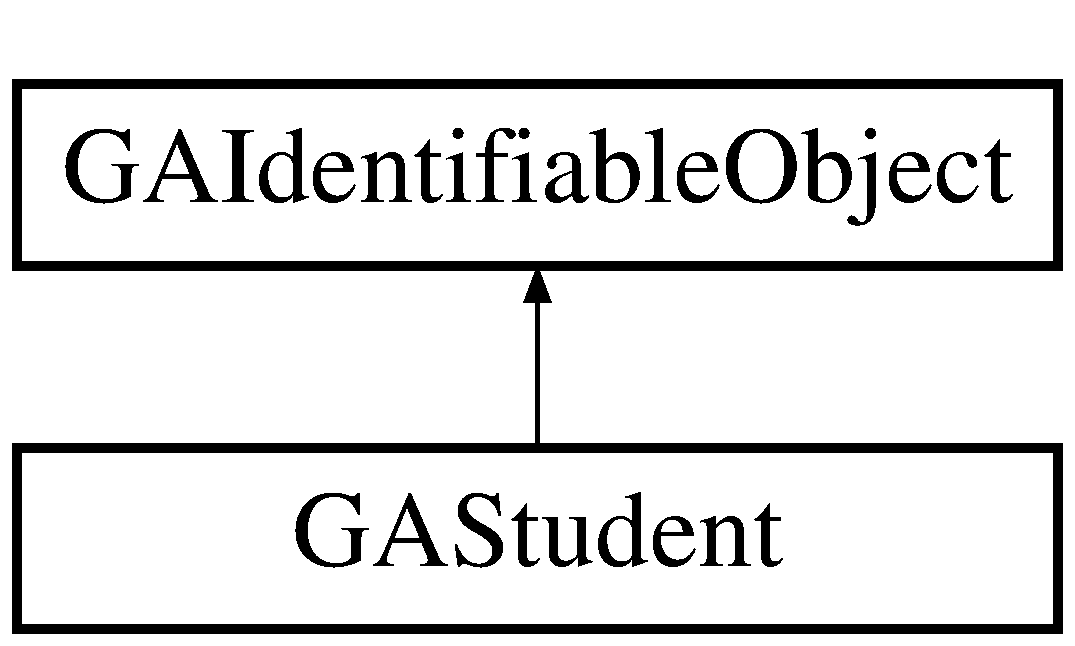
\includegraphics[height=2.000000cm]{class_g_a_student}
\end{center}
\end{figure}
\subsection*{Public Member Functions}
\begin{DoxyCompactItemize}
\item 
\hyperlink{class_g_a_student_a83c98a132e18c6f630028f3ee4e94fb2}{G\+A\+Student} (std\+::string name, std\+::string laf\+\_\+id)
\begin{DoxyCompactList}\small\item\em Construct a \hyperlink{class_g_a_student}{G\+A\+Student}. \end{DoxyCompactList}\item 
\hyperlink{class_g_a_student_a781128a3ff0098a7df81760c6ea8d9c8}{G\+A\+Student} (std\+::string id, std\+::string name, std\+::string laf\+\_\+id)
\begin{DoxyCompactList}\small\item\em Construct a \hyperlink{class_g_a_student}{G\+A\+Student} with a provided persistence ID. \end{DoxyCompactList}\item 
virtual \hyperlink{class_g_a_student_a8bf2b66d9d4bf773d903d8e0c26faf22}{$\sim$\+G\+A\+Student} ()
\begin{DoxyCompactList}\small\item\em Deconstruct a \hyperlink{class_g_a_student}{G\+A\+Student}. \end{DoxyCompactList}\item 
std\+::string \hyperlink{class_g_a_student_a2424100663a950f60d02b70b00610dde}{get\+\_\+name} ()
\begin{DoxyCompactList}\small\item\em Get the name of the student. \end{DoxyCompactList}\item 
void \hyperlink{class_g_a_student_ab8224579ce2618e60455a8a73b1473f9}{set\+\_\+name} (std\+::string name)
\begin{DoxyCompactList}\small\item\em Set the name of the student. \end{DoxyCompactList}\item 
std\+::string \hyperlink{class_g_a_student_ad3f1ce3ab268f13812fbf126a2ca018a}{get\+\_\+lafayette\+\_\+username} ()
\begin{DoxyCompactList}\small\item\em Get the Lafayette username of the student. \end{DoxyCompactList}\item 
void \hyperlink{class_g_a_student_a996265e95742082a4f762b2fe6022c65}{set\+\_\+lafayette\+\_\+username} (std\+::string username)
\begin{DoxyCompactList}\small\item\em Set the Lafayette username of the student. \end{DoxyCompactList}\item 
\hyperlink{class_g_a_class}{G\+A\+Class} $\ast$ \hyperlink{class_g_a_student_ad0cdfa58f5b581d0e5d671e402dc7127}{get\+\_\+class} ()
\begin{DoxyCompactList}\small\item\em Get the \hyperlink{class_g_a_class}{G\+A\+Class} the student is enrolled in. \end{DoxyCompactList}\item 
void \hyperlink{class_g_a_student_a032086c71e6852d47c3204c10ac481e3}{set\+\_\+class} (\hyperlink{class_g_a_class}{G\+A\+Class} $\ast$class\+\_\+)
\begin{DoxyCompactList}\small\item\em Set the \hyperlink{class_g_a_class}{G\+A\+Class} the student is enrolled in. \end{DoxyCompactList}\item 
void \hyperlink{class_g_a_student_a4cc7c39cf2d032023e6cd5e6313152c7}{set\+\_\+data} (\hyperlink{class_g_a_assignment}{G\+A\+Assignment} $\ast$a, \hyperlink{class_g_a_assignment_data}{G\+A\+Assignment\+Data} $\ast$d)
\begin{DoxyCompactList}\small\item\em Set the assignment data object. \end{DoxyCompactList}\item 
\hyperlink{class_g_a_assignment_data}{G\+A\+Assignment\+Data} $\ast$ \hyperlink{class_g_a_student_a95bb10e02192cd098323b313a4155827}{get\+\_\+data} (\hyperlink{class_g_a_assignment}{G\+A\+Assignment} $\ast$a)
\begin{DoxyCompactList}\small\item\em Get the assignment data object. \end{DoxyCompactList}\item 
std\+::map$<$ \hyperlink{class_g_a_assignment}{G\+A\+Assignment} $\ast$, \hyperlink{class_g_a_assignment_data}{G\+A\+Assignment\+Data} $\ast$ $>$ \hyperlink{class_g_a_student_a967fe8dc4aac505d1a6dbc8535736681}{get\+\_\+map} ()
\begin{DoxyCompactList}\small\item\em Get the \hyperlink{class_g_a_assignment}{G\+A\+Assignment} -\/ \hyperlink{class_g_a_assignment_data}{G\+A\+Assignment\+Data} map. \end{DoxyCompactList}\item 
bool \hyperlink{class_g_a_student_a752f52729e51c7b3b31d86a3e812088b}{save\+\_\+to} (\hyperlink{class_database_table}{Database\+Table} $\ast$table)
\begin{DoxyCompactList}\small\item\em Save this object to a table. \end{DoxyCompactList}\item 
void \hyperlink{class_g_a_student_a35c859da932a8a83f5622bcd46ae1269}{remove\+\_\+from} (\hyperlink{class_database_table}{Database\+Table} $\ast$table)
\begin{DoxyCompactList}\small\item\em Remove this object from a table. \end{DoxyCompactList}\end{DoxyCompactItemize}
\subsection*{Static Public Member Functions}
\begin{DoxyCompactItemize}
\item 
static std\+::vector$<$ \hyperlink{class_g_a_student}{G\+A\+Student} $\ast$ $>$ \hyperlink{class_g_a_student_a7b95740499af16d32f2b12ec2508ee7e}{load\+\_\+from} (\hyperlink{class_database_table}{Database\+Table} $\ast$table, \hyperlink{class_g_a_class}{G\+A\+Class} $\ast$class\+\_\+)
\begin{DoxyCompactList}\small\item\em Load all students from a table (who are enrolled in a specific class) \end{DoxyCompactList}\end{DoxyCompactItemize}


\subsection{Constructor \& Destructor Documentation}
\mbox{\Hypertarget{class_g_a_student_a83c98a132e18c6f630028f3ee4e94fb2}\label{class_g_a_student_a83c98a132e18c6f630028f3ee4e94fb2}} 
\index{G\+A\+Student@{G\+A\+Student}!G\+A\+Student@{G\+A\+Student}}
\index{G\+A\+Student@{G\+A\+Student}!G\+A\+Student@{G\+A\+Student}}
\subsubsection{\texorpdfstring{G\+A\+Student()}{GAStudent()}\hspace{0.1cm}{\footnotesize\ttfamily [1/2]}}
{\footnotesize\ttfamily G\+A\+Student\+::\+G\+A\+Student (\begin{DoxyParamCaption}\item[{std\+::string}]{name,  }\item[{std\+::string}]{laf\+\_\+id }\end{DoxyParamCaption})}



Construct a \hyperlink{class_g_a_student}{G\+A\+Student}. 


\begin{DoxyParams}{Parameters}
{\em name} & The name for the student \\
\hline
{\em laf\+\_\+id} & The Lafayette username for the student (not their student ID) \\
\hline
\end{DoxyParams}
\mbox{\Hypertarget{class_g_a_student_a781128a3ff0098a7df81760c6ea8d9c8}\label{class_g_a_student_a781128a3ff0098a7df81760c6ea8d9c8}} 
\index{G\+A\+Student@{G\+A\+Student}!G\+A\+Student@{G\+A\+Student}}
\index{G\+A\+Student@{G\+A\+Student}!G\+A\+Student@{G\+A\+Student}}
\subsubsection{\texorpdfstring{G\+A\+Student()}{GAStudent()}\hspace{0.1cm}{\footnotesize\ttfamily [2/2]}}
{\footnotesize\ttfamily G\+A\+Student\+::\+G\+A\+Student (\begin{DoxyParamCaption}\item[{std\+::string}]{id,  }\item[{std\+::string}]{name,  }\item[{std\+::string}]{laf\+\_\+id }\end{DoxyParamCaption})}



Construct a \hyperlink{class_g_a_student}{G\+A\+Student} with a provided persistence ID. 


\begin{DoxyParams}{Parameters}
{\em id} & The ID to use \\
\hline
{\em name} & The name for the student \\
\hline
{\em laf\+\_\+id} & The Lafayette username for the student (not their student ID) \\
\hline
\end{DoxyParams}
\mbox{\Hypertarget{class_g_a_student_a8bf2b66d9d4bf773d903d8e0c26faf22}\label{class_g_a_student_a8bf2b66d9d4bf773d903d8e0c26faf22}} 
\index{G\+A\+Student@{G\+A\+Student}!````~G\+A\+Student@{$\sim$\+G\+A\+Student}}
\index{````~G\+A\+Student@{$\sim$\+G\+A\+Student}!G\+A\+Student@{G\+A\+Student}}
\subsubsection{\texorpdfstring{$\sim$\+G\+A\+Student()}{~GAStudent()}}
{\footnotesize\ttfamily G\+A\+Student\+::$\sim$\+G\+A\+Student (\begin{DoxyParamCaption}{ }\end{DoxyParamCaption})\hspace{0.3cm}{\ttfamily [virtual]}}



Deconstruct a \hyperlink{class_g_a_student}{G\+A\+Student}. 

This will remove all the Assignment\+Data objects, which are owned by the \hyperlink{class_g_a_student}{G\+A\+Student} objects 

\subsection{Member Function Documentation}
\mbox{\Hypertarget{class_g_a_student_ad0cdfa58f5b581d0e5d671e402dc7127}\label{class_g_a_student_ad0cdfa58f5b581d0e5d671e402dc7127}} 
\index{G\+A\+Student@{G\+A\+Student}!get\+\_\+class@{get\+\_\+class}}
\index{get\+\_\+class@{get\+\_\+class}!G\+A\+Student@{G\+A\+Student}}
\subsubsection{\texorpdfstring{get\+\_\+class()}{get\_class()}}
{\footnotesize\ttfamily \hyperlink{class_g_a_class}{G\+A\+Class} $\ast$ G\+A\+Student\+::get\+\_\+class (\begin{DoxyParamCaption}{ }\end{DoxyParamCaption})}



Get the \hyperlink{class_g_a_class}{G\+A\+Class} the student is enrolled in. 

\begin{DoxyReturn}{Returns}
The class 
\end{DoxyReturn}
\mbox{\Hypertarget{class_g_a_student_a95bb10e02192cd098323b313a4155827}\label{class_g_a_student_a95bb10e02192cd098323b313a4155827}} 
\index{G\+A\+Student@{G\+A\+Student}!get\+\_\+data@{get\+\_\+data}}
\index{get\+\_\+data@{get\+\_\+data}!G\+A\+Student@{G\+A\+Student}}
\subsubsection{\texorpdfstring{get\+\_\+data()}{get\_data()}}
{\footnotesize\ttfamily \hyperlink{class_g_a_assignment_data}{G\+A\+Assignment\+Data} $\ast$ G\+A\+Student\+::get\+\_\+data (\begin{DoxyParamCaption}\item[{\hyperlink{class_g_a_assignment}{G\+A\+Assignment} $\ast$}]{a }\end{DoxyParamCaption})}



Get the assignment data object. 

This will not return nullptr unless the student is not in the class the assignment is associated with


\begin{DoxyParams}{Parameters}
{\em a} & The assignment \\
\hline
\end{DoxyParams}
\begin{DoxyReturn}{Returns}
The assignment data 
\end{DoxyReturn}
\mbox{\Hypertarget{class_g_a_student_ad3f1ce3ab268f13812fbf126a2ca018a}\label{class_g_a_student_ad3f1ce3ab268f13812fbf126a2ca018a}} 
\index{G\+A\+Student@{G\+A\+Student}!get\+\_\+lafayette\+\_\+username@{get\+\_\+lafayette\+\_\+username}}
\index{get\+\_\+lafayette\+\_\+username@{get\+\_\+lafayette\+\_\+username}!G\+A\+Student@{G\+A\+Student}}
\subsubsection{\texorpdfstring{get\+\_\+lafayette\+\_\+username()}{get\_lafayette\_username()}}
{\footnotesize\ttfamily std\+::string G\+A\+Student\+::get\+\_\+lafayette\+\_\+username (\begin{DoxyParamCaption}{ }\end{DoxyParamCaption})}



Get the Lafayette username of the student. 

\begin{DoxyReturn}{Returns}
The Lafayette username 
\end{DoxyReturn}
\mbox{\Hypertarget{class_g_a_student_a967fe8dc4aac505d1a6dbc8535736681}\label{class_g_a_student_a967fe8dc4aac505d1a6dbc8535736681}} 
\index{G\+A\+Student@{G\+A\+Student}!get\+\_\+map@{get\+\_\+map}}
\index{get\+\_\+map@{get\+\_\+map}!G\+A\+Student@{G\+A\+Student}}
\subsubsection{\texorpdfstring{get\+\_\+map()}{get\_map()}}
{\footnotesize\ttfamily std\+::map$<$ \hyperlink{class_g_a_assignment}{G\+A\+Assignment} $\ast$, \hyperlink{class_g_a_assignment_data}{G\+A\+Assignment\+Data} $\ast$ $>$ G\+A\+Student\+::get\+\_\+map (\begin{DoxyParamCaption}{ }\end{DoxyParamCaption})}



Get the \hyperlink{class_g_a_assignment}{G\+A\+Assignment} -\/ \hyperlink{class_g_a_assignment_data}{G\+A\+Assignment\+Data} map. 

\begin{DoxyReturn}{Returns}
The map 
\end{DoxyReturn}
\mbox{\Hypertarget{class_g_a_student_a2424100663a950f60d02b70b00610dde}\label{class_g_a_student_a2424100663a950f60d02b70b00610dde}} 
\index{G\+A\+Student@{G\+A\+Student}!get\+\_\+name@{get\+\_\+name}}
\index{get\+\_\+name@{get\+\_\+name}!G\+A\+Student@{G\+A\+Student}}
\subsubsection{\texorpdfstring{get\+\_\+name()}{get\_name()}}
{\footnotesize\ttfamily std\+::string G\+A\+Student\+::get\+\_\+name (\begin{DoxyParamCaption}{ }\end{DoxyParamCaption})}



Get the name of the student. 

\begin{DoxyReturn}{Returns}
The name of the student 
\end{DoxyReturn}
\mbox{\Hypertarget{class_g_a_student_a7b95740499af16d32f2b12ec2508ee7e}\label{class_g_a_student_a7b95740499af16d32f2b12ec2508ee7e}} 
\index{G\+A\+Student@{G\+A\+Student}!load\+\_\+from@{load\+\_\+from}}
\index{load\+\_\+from@{load\+\_\+from}!G\+A\+Student@{G\+A\+Student}}
\subsubsection{\texorpdfstring{load\+\_\+from()}{load\_from()}}
{\footnotesize\ttfamily std\+::vector$<$ \hyperlink{class_g_a_student}{G\+A\+Student} $\ast$ $>$ G\+A\+Student\+::load\+\_\+from (\begin{DoxyParamCaption}\item[{\hyperlink{class_database_table}{Database\+Table} $\ast$}]{table,  }\item[{\hyperlink{class_g_a_class}{G\+A\+Class} $\ast$}]{class\+\_\+ }\end{DoxyParamCaption})\hspace{0.3cm}{\ttfamily [static]}}



Load all students from a table (who are enrolled in a specific class) 


\begin{DoxyParams}{Parameters}
{\em table} & The table \\
\hline
{\em class\+\_\+} & The class \\
\hline
\end{DoxyParams}
\begin{DoxyReturn}{Returns}
The student vector 
\end{DoxyReturn}
\mbox{\Hypertarget{class_g_a_student_a35c859da932a8a83f5622bcd46ae1269}\label{class_g_a_student_a35c859da932a8a83f5622bcd46ae1269}} 
\index{G\+A\+Student@{G\+A\+Student}!remove\+\_\+from@{remove\+\_\+from}}
\index{remove\+\_\+from@{remove\+\_\+from}!G\+A\+Student@{G\+A\+Student}}
\subsubsection{\texorpdfstring{remove\+\_\+from()}{remove\_from()}}
{\footnotesize\ttfamily void G\+A\+Student\+::remove\+\_\+from (\begin{DoxyParamCaption}\item[{\hyperlink{class_database_table}{Database\+Table} $\ast$}]{table }\end{DoxyParamCaption})}



Remove this object from a table. 


\begin{DoxyParams}{Parameters}
{\em table} & The table \\
\hline
\end{DoxyParams}
\mbox{\Hypertarget{class_g_a_student_a752f52729e51c7b3b31d86a3e812088b}\label{class_g_a_student_a752f52729e51c7b3b31d86a3e812088b}} 
\index{G\+A\+Student@{G\+A\+Student}!save\+\_\+to@{save\+\_\+to}}
\index{save\+\_\+to@{save\+\_\+to}!G\+A\+Student@{G\+A\+Student}}
\subsubsection{\texorpdfstring{save\+\_\+to()}{save\_to()}}
{\footnotesize\ttfamily bool G\+A\+Student\+::save\+\_\+to (\begin{DoxyParamCaption}\item[{\hyperlink{class_database_table}{Database\+Table} $\ast$}]{table }\end{DoxyParamCaption})}



Save this object to a table. 


\begin{DoxyParams}{Parameters}
{\em table} & The table \\
\hline
\end{DoxyParams}
\begin{DoxyReturn}{Returns}
Whether the insert was successful 
\end{DoxyReturn}
\mbox{\Hypertarget{class_g_a_student_a032086c71e6852d47c3204c10ac481e3}\label{class_g_a_student_a032086c71e6852d47c3204c10ac481e3}} 
\index{G\+A\+Student@{G\+A\+Student}!set\+\_\+class@{set\+\_\+class}}
\index{set\+\_\+class@{set\+\_\+class}!G\+A\+Student@{G\+A\+Student}}
\subsubsection{\texorpdfstring{set\+\_\+class()}{set\_class()}}
{\footnotesize\ttfamily void G\+A\+Student\+::set\+\_\+class (\begin{DoxyParamCaption}\item[{\hyperlink{class_g_a_class}{G\+A\+Class} $\ast$}]{class\+\_\+ }\end{DoxyParamCaption})}



Set the \hyperlink{class_g_a_class}{G\+A\+Class} the student is enrolled in. 


\begin{DoxyParams}{Parameters}
{\em class\+\_\+} & The class \\
\hline
\end{DoxyParams}
\mbox{\Hypertarget{class_g_a_student_a4cc7c39cf2d032023e6cd5e6313152c7}\label{class_g_a_student_a4cc7c39cf2d032023e6cd5e6313152c7}} 
\index{G\+A\+Student@{G\+A\+Student}!set\+\_\+data@{set\+\_\+data}}
\index{set\+\_\+data@{set\+\_\+data}!G\+A\+Student@{G\+A\+Student}}
\subsubsection{\texorpdfstring{set\+\_\+data()}{set\_data()}}
{\footnotesize\ttfamily void G\+A\+Student\+::set\+\_\+data (\begin{DoxyParamCaption}\item[{\hyperlink{class_g_a_assignment}{G\+A\+Assignment} $\ast$}]{a,  }\item[{\hyperlink{class_g_a_assignment_data}{G\+A\+Assignment\+Data} $\ast$}]{d }\end{DoxyParamCaption})}



Set the assignment data object. 

Do not create an assignment data object, instead call get\+\_\+data(\+G\+A\+Assignment\+Data$\ast$ a) to get a properly linked object.


\begin{DoxyParams}{Parameters}
{\em a} & The \hyperlink{class_g_a_assignment}{G\+A\+Assignment} \\
\hline
{\em d} & The \hyperlink{class_g_a_assignment_data}{G\+A\+Assignment\+Data} \\
\hline
\end{DoxyParams}
\mbox{\Hypertarget{class_g_a_student_a996265e95742082a4f762b2fe6022c65}\label{class_g_a_student_a996265e95742082a4f762b2fe6022c65}} 
\index{G\+A\+Student@{G\+A\+Student}!set\+\_\+lafayette\+\_\+username@{set\+\_\+lafayette\+\_\+username}}
\index{set\+\_\+lafayette\+\_\+username@{set\+\_\+lafayette\+\_\+username}!G\+A\+Student@{G\+A\+Student}}
\subsubsection{\texorpdfstring{set\+\_\+lafayette\+\_\+username()}{set\_lafayette\_username()}}
{\footnotesize\ttfamily void G\+A\+Student\+::set\+\_\+lafayette\+\_\+username (\begin{DoxyParamCaption}\item[{std\+::string}]{username }\end{DoxyParamCaption})}



Set the Lafayette username of the student. 


\begin{DoxyParams}{Parameters}
{\em username} & The Lafayette username \\
\hline
\end{DoxyParams}
\mbox{\Hypertarget{class_g_a_student_ab8224579ce2618e60455a8a73b1473f9}\label{class_g_a_student_ab8224579ce2618e60455a8a73b1473f9}} 
\index{G\+A\+Student@{G\+A\+Student}!set\+\_\+name@{set\+\_\+name}}
\index{set\+\_\+name@{set\+\_\+name}!G\+A\+Student@{G\+A\+Student}}
\subsubsection{\texorpdfstring{set\+\_\+name()}{set\_name()}}
{\footnotesize\ttfamily void G\+A\+Student\+::set\+\_\+name (\begin{DoxyParamCaption}\item[{std\+::string}]{name }\end{DoxyParamCaption})}



Set the name of the student. 


\begin{DoxyParams}{Parameters}
{\em name} & The name of the student \\
\hline
\end{DoxyParams}


The documentation for this class was generated from the following files\+:\begin{DoxyCompactItemize}
\item 
grading-\/assistant/gadata/gastudent.\+h\item 
grading-\/assistant/gadata/gastudent.\+cpp\end{DoxyCompactItemize}

\hypertarget{class_grading_assistant}{}\section{Grading\+Assistant Class Reference}
\label{class_grading_assistant}\index{Grading\+Assistant@{Grading\+Assistant}}
\subsection*{Public Member Functions}
\begin{DoxyCompactItemize}
\item 
\hyperlink{class_grading_assistant_af3831409f51b90db892b366527742f01}{Grading\+Assistant} (\hyperlink{class_database_manager}{Database\+Manager} $\ast$database)
\begin{DoxyCompactList}\small\item\em Create a \hyperlink{class_grading_assistant}{Grading\+Assistant}. \end{DoxyCompactList}\item 
\hyperlink{class_grading_assistant_a8bc628e497b2f818fdc97c2e8eb5e26f}{$\sim$\+Grading\+Assistant} ()
\begin{DoxyCompactList}\small\item\em Deconstruct the \hyperlink{class_grading_assistant}{Grading\+Assistant} object. \end{DoxyCompactList}\item 
std\+::vector$<$ \hyperlink{class_g_a_class}{G\+A\+Class} $\ast$ $>$ \hyperlink{class_grading_assistant_af386f98b366cae34c8761f8c133f9eb9}{get\+\_\+classes} ()
\begin{DoxyCompactList}\small\item\em Get the \hyperlink{class_g_a_class}{G\+A\+Class} vector. \end{DoxyCompactList}\item 
void \hyperlink{class_grading_assistant_a5bbda42e70ff9c9a7fe9cadcf58681bd}{add\+\_\+class} (\hyperlink{class_g_a_class}{G\+A\+Class} $\ast$c)
\begin{DoxyCompactList}\small\item\em Add a \hyperlink{class_g_a_class}{G\+A\+Class}. \end{DoxyCompactList}\item 
std\+::vector$<$ \hyperlink{class_g_a_rubric}{G\+A\+Rubric} $\ast$ $>$ \hyperlink{class_grading_assistant_a05211ce3152422e668e6afeb5f9726bb}{get\+\_\+rubrics} ()
\begin{DoxyCompactList}\small\item\em Get the \hyperlink{class_g_a_rubric}{G\+A\+Rubric} vector. \end{DoxyCompactList}\item 
void \hyperlink{class_grading_assistant_ad072b785eb9fc6b174e0129f4cf3697a}{add\+\_\+rubric} (\hyperlink{class_g_a_rubric}{G\+A\+Rubric} $\ast$r)
\begin{DoxyCompactList}\small\item\em Add a \hyperlink{class_g_a_rubric}{G\+A\+Rubric}. \end{DoxyCompactList}\item 
void \hyperlink{class_grading_assistant_ae4d29640f6444cc59d7df5eb73f60115}{save} ()
\begin{DoxyCompactList}\small\item\em Save all the data. \end{DoxyCompactList}\item 
void \hyperlink{class_grading_assistant_a2430309557f1fd413a75165b4c7c9a3a}{load} ()
\begin{DoxyCompactList}\small\item\em Load the data. \end{DoxyCompactList}\end{DoxyCompactItemize}


\subsection{Constructor \& Destructor Documentation}
\mbox{\Hypertarget{class_grading_assistant_af3831409f51b90db892b366527742f01}\label{class_grading_assistant_af3831409f51b90db892b366527742f01}} 
\index{Grading\+Assistant@{Grading\+Assistant}!Grading\+Assistant@{Grading\+Assistant}}
\index{Grading\+Assistant@{Grading\+Assistant}!Grading\+Assistant@{Grading\+Assistant}}
\subsubsection{\texorpdfstring{Grading\+Assistant()}{GradingAssistant()}}
{\footnotesize\ttfamily Grading\+Assistant\+::\+Grading\+Assistant (\begin{DoxyParamCaption}\item[{\hyperlink{class_database_manager}{Database\+Manager} $\ast$}]{database }\end{DoxyParamCaption})}



Create a \hyperlink{class_grading_assistant}{Grading\+Assistant}. 

The initalizer defines all the tables, but does not load anything


\begin{DoxyParams}{Parameters}
{\em database} & The database to use \\
\hline
\end{DoxyParams}
\mbox{\Hypertarget{class_grading_assistant_a8bc628e497b2f818fdc97c2e8eb5e26f}\label{class_grading_assistant_a8bc628e497b2f818fdc97c2e8eb5e26f}} 
\index{Grading\+Assistant@{Grading\+Assistant}!````~Grading\+Assistant@{$\sim$\+Grading\+Assistant}}
\index{````~Grading\+Assistant@{$\sim$\+Grading\+Assistant}!Grading\+Assistant@{Grading\+Assistant}}
\subsubsection{\texorpdfstring{$\sim$\+Grading\+Assistant()}{~GradingAssistant()}}
{\footnotesize\ttfamily Grading\+Assistant\+::$\sim$\+Grading\+Assistant (\begin{DoxyParamCaption}{ }\end{DoxyParamCaption})}



Deconstruct the \hyperlink{class_grading_assistant}{Grading\+Assistant} object. 

This will delete all the classes, rubrics, and tables from memory 

\subsection{Member Function Documentation}
\mbox{\Hypertarget{class_grading_assistant_a5bbda42e70ff9c9a7fe9cadcf58681bd}\label{class_grading_assistant_a5bbda42e70ff9c9a7fe9cadcf58681bd}} 
\index{Grading\+Assistant@{Grading\+Assistant}!add\+\_\+class@{add\+\_\+class}}
\index{add\+\_\+class@{add\+\_\+class}!Grading\+Assistant@{Grading\+Assistant}}
\subsubsection{\texorpdfstring{add\+\_\+class()}{add\_class()}}
{\footnotesize\ttfamily void Grading\+Assistant\+::add\+\_\+class (\begin{DoxyParamCaption}\item[{\hyperlink{class_g_a_class}{G\+A\+Class} $\ast$}]{c }\end{DoxyParamCaption})}



Add a \hyperlink{class_g_a_class}{G\+A\+Class}. 


\begin{DoxyParams}{Parameters}
{\em c} & The \hyperlink{class_g_a_class}{G\+A\+Class} to add \\
\hline
\end{DoxyParams}
\mbox{\Hypertarget{class_grading_assistant_ad072b785eb9fc6b174e0129f4cf3697a}\label{class_grading_assistant_ad072b785eb9fc6b174e0129f4cf3697a}} 
\index{Grading\+Assistant@{Grading\+Assistant}!add\+\_\+rubric@{add\+\_\+rubric}}
\index{add\+\_\+rubric@{add\+\_\+rubric}!Grading\+Assistant@{Grading\+Assistant}}
\subsubsection{\texorpdfstring{add\+\_\+rubric()}{add\_rubric()}}
{\footnotesize\ttfamily void Grading\+Assistant\+::add\+\_\+rubric (\begin{DoxyParamCaption}\item[{\hyperlink{class_g_a_rubric}{G\+A\+Rubric} $\ast$}]{r }\end{DoxyParamCaption})}



Add a \hyperlink{class_g_a_rubric}{G\+A\+Rubric}. 


\begin{DoxyParams}{Parameters}
{\em r} & The \hyperlink{class_g_a_rubric}{G\+A\+Rubric} to add \\
\hline
\end{DoxyParams}
\mbox{\Hypertarget{class_grading_assistant_af386f98b366cae34c8761f8c133f9eb9}\label{class_grading_assistant_af386f98b366cae34c8761f8c133f9eb9}} 
\index{Grading\+Assistant@{Grading\+Assistant}!get\+\_\+classes@{get\+\_\+classes}}
\index{get\+\_\+classes@{get\+\_\+classes}!Grading\+Assistant@{Grading\+Assistant}}
\subsubsection{\texorpdfstring{get\+\_\+classes()}{get\_classes()}}
{\footnotesize\ttfamily std\+::vector$<$ \hyperlink{class_g_a_class}{G\+A\+Class} $\ast$ $>$ Grading\+Assistant\+::get\+\_\+classes (\begin{DoxyParamCaption}{ }\end{DoxyParamCaption})}



Get the \hyperlink{class_g_a_class}{G\+A\+Class} vector. 

\begin{DoxyReturn}{Returns}
The \hyperlink{class_g_a_class}{G\+A\+Class} vector 
\end{DoxyReturn}
\mbox{\Hypertarget{class_grading_assistant_a05211ce3152422e668e6afeb5f9726bb}\label{class_grading_assistant_a05211ce3152422e668e6afeb5f9726bb}} 
\index{Grading\+Assistant@{Grading\+Assistant}!get\+\_\+rubrics@{get\+\_\+rubrics}}
\index{get\+\_\+rubrics@{get\+\_\+rubrics}!Grading\+Assistant@{Grading\+Assistant}}
\subsubsection{\texorpdfstring{get\+\_\+rubrics()}{get\_rubrics()}}
{\footnotesize\ttfamily std\+::vector$<$ \hyperlink{class_g_a_rubric}{G\+A\+Rubric} $\ast$ $>$ Grading\+Assistant\+::get\+\_\+rubrics (\begin{DoxyParamCaption}{ }\end{DoxyParamCaption})}



Get the \hyperlink{class_g_a_rubric}{G\+A\+Rubric} vector. 

\begin{DoxyReturn}{Returns}
The \hyperlink{class_g_a_rubric}{G\+A\+Rubric} vector 
\end{DoxyReturn}
\mbox{\Hypertarget{class_grading_assistant_a2430309557f1fd413a75165b4c7c9a3a}\label{class_grading_assistant_a2430309557f1fd413a75165b4c7c9a3a}} 
\index{Grading\+Assistant@{Grading\+Assistant}!load@{load}}
\index{load@{load}!Grading\+Assistant@{Grading\+Assistant}}
\subsubsection{\texorpdfstring{load()}{load()}}
{\footnotesize\ttfamily void Grading\+Assistant\+::load (\begin{DoxyParamCaption}{ }\end{DoxyParamCaption})}



Load the data. 

This will not currently clear the existing data in memory. The \hyperlink{class_grading_assistant}{Grading\+Assistant} object should be initialized prior to running this. \mbox{\Hypertarget{class_grading_assistant_ae4d29640f6444cc59d7df5eb73f60115}\label{class_grading_assistant_ae4d29640f6444cc59d7df5eb73f60115}} 
\index{Grading\+Assistant@{Grading\+Assistant}!save@{save}}
\index{save@{save}!Grading\+Assistant@{Grading\+Assistant}}
\subsubsection{\texorpdfstring{save()}{save()}}
{\footnotesize\ttfamily void Grading\+Assistant\+::save (\begin{DoxyParamCaption}{ }\end{DoxyParamCaption})}



Save all the data. 

This will clear all the tables, then go through all the objects and save them 

The documentation for this class was generated from the following files\+:\begin{DoxyCompactItemize}
\item 
grading-\/assistant/gradingassistant.\+h\item 
grading-\/assistant/gradingassistant.\+cpp\end{DoxyCompactItemize}

\hypertarget{class_user_settings}{}\section{User\+Settings Class Reference}
\label{class_user_settings}\index{User\+Settings@{User\+Settings}}
\subsection*{Public Member Functions}
\begin{DoxyCompactItemize}
\item 
\mbox{\Hypertarget{class_user_settings_ab8ce58827355048f7b397d95c3d3d421}\label{class_user_settings_ab8ce58827355048f7b397d95c3d3d421}} 
{\bfseries User\+Settings} (std\+::string path)
\item 
\mbox{\Hypertarget{class_user_settings_afa1dddce37e80cdd7444a22716ed11fd}\label{class_user_settings_afa1dddce37e80cdd7444a22716ed11fd}} 
{\bfseries User\+Settings} (\hyperlink{class_user_settings}{User\+Settings} \&obj)
\item 
\mbox{\Hypertarget{class_user_settings_a3dcfa0b162d84538de39e8f03267858a}\label{class_user_settings_a3dcfa0b162d84538de39e8f03267858a}} 
void {\bfseries operator=} (\hyperlink{class_user_settings}{User\+Settings} \&obj)
\item 
\mbox{\Hypertarget{class_user_settings_af6354aa4cad29e254e7acce48425f9ba}\label{class_user_settings_af6354aa4cad29e254e7acce48425f9ba}} 
void {\bfseries save} ()
\item 
\mbox{\Hypertarget{class_user_settings_a893482525be333465128a6896593e651}\label{class_user_settings_a893482525be333465128a6896593e651}} 
void {\bfseries load} ()
\item 
\mbox{\Hypertarget{class_user_settings_a8b3bc0132ec9dbc8a8bb5f91194a9593}\label{class_user_settings_a8b3bc0132ec9dbc8a8bb5f91194a9593}} 
std\+::string {\bfseries get\+\_\+path} ()
\item 
\mbox{\Hypertarget{class_user_settings_ab45dc788b479df11ce40414333f8e7c8}\label{class_user_settings_ab45dc788b479df11ce40414333f8e7c8}} 
void {\bfseries set\+\_\+path} (std\+::string path)
\item 
\mbox{\Hypertarget{class_user_settings_a9c74c02c3b62d39f4733f9e2bb7ea71d}\label{class_user_settings_a9c74c02c3b62d39f4733f9e2bb7ea71d}} 
void {\bfseries set} (std\+::string key, std\+::string value)
\item 
\mbox{\Hypertarget{class_user_settings_ac963d1939ddf67ac594e31f8cd63a183}\label{class_user_settings_ac963d1939ddf67ac594e31f8cd63a183}} 
std\+::string {\bfseries get\+String} (std\+::string key)
\item 
\mbox{\Hypertarget{class_user_settings_a087db56471b446fd4fddf1a0e2c8be1a}\label{class_user_settings_a087db56471b446fd4fddf1a0e2c8be1a}} 
void {\bfseries set} (std\+::string key, int value)
\item 
\mbox{\Hypertarget{class_user_settings_a90d70b27fcf3f9c611c9db108edd18e5}\label{class_user_settings_a90d70b27fcf3f9c611c9db108edd18e5}} 
int {\bfseries get\+Int} (std\+::string key)
\end{DoxyCompactItemize}


The documentation for this class was generated from the following files\+:\begin{DoxyCompactItemize}
\item 
grading-\/assistant/usersettings.\+h\item 
grading-\/assistant/usersettings.\+cpp\end{DoxyCompactItemize}

%--- End generated contents ---

% Index
\backmatter
\newpage
\phantomsection
\clearemptydoublepage
\addcontentsline{toc}{chapter}{Index}
\printindex

\end{document}
